%\setchapterpreamble[u]{\margintoc}
\chapter{Linguaggi Regolari}\label{cha:Linguaggi-regolari}




\section{Introduzione}\label{sec:regolari-introduzione}

In questo caso vogliamo identificare una classe di linguaggi che sia semplice da definire, che ammetta un riconoscitore
efficiente, ma non sia così ristretta da ammettere solo linguaggi banali.
Per ottenere questo obiettivo, introduciamo le espressioni regolari che portano ad una definizione di tipo
insiemistico dei linguaggi regolari.

\begin{definition}[espressione regolare]\label{def:regex}
Sia $\Sigma$ un alfabeto. Un'\keyword{espressione regolare} è definita secondo le seguenti regole.
\begin{enumerate}
\item $\varepsilon$ e $\emptyset$ sono espressioni regolari;
\item Ogni simbolo $\sigma\in\Sigma$ è un'espressione regolare;
\item Se $E_1$ e $E_2$ sono due espressioni regolari, allora $E_1 \cup E_2$ è un'espressione regolare corrispondente
	  all'unione, o alternanza, fra $E_1$ e $E_2$;
\item Se $E_1$ e $E_2$ sono due espressioni regolari, allora $E_1 E_2$ è un'espressione regolare corrispondente
	  alla concatenazione di $E_1$ e $E_2$;
\item Se $E$ è un'espressione regolare, allora $E_1^{*}$ è un'espressione regolare corrispondente
	  alla chiusura di Kleene di $E$, ovvero alla ripetizione di $E$ un numero imprecisato (incluso $0$) di volte;
\item Se $E$ è un'espressione regolare, allora $(E)$ è un'espressione regolare.
\end{enumerate}
\end{definition}

Le operazioni hanno un ordine di precedenza di valutazione (a parità di precedenza, si valuta da sinistra a destra), in
ordine descrescente di precedenza:
\begin{enumerate}
	\item parentesi
	\item chiusura di Kleene *
	\item concatenazione
	\item unione
\end{enumerate}


Notiamo che le espressioni regolari sono una sintassi che, al momento, può apparire priva di significato concreto.
Abbiamo bisogno di introdurre il linguaggio associato ad un'espressione regolare, seguendo pedissequamente i casi della \Cref{def:regex}.

\begin{definition}[Linguaggio associato ad un'espressione regolare]\label{def:regex-linguaggio}
Sia $E$ un'espressione regolare. Il linguaggio $L(E)$ associato a $E$ è definito secondo le seguenti regole.
\begin{enumerate}
	  \item $L(\epsilon) = \{\epsilon\}$, $L(\emptyset) = \emptyset$;
\item Se $E$ consiste unicamente di un simbolo $\sigma\in\Sigma$, allora $L(E) = \{\sigma\}$;
\item Se $E=E_1 \cup E_2$, allora $L(E) = \{w\in \Sigma^{*} : w\in L(E_{1}) \vee  w\in L(E_{2})\}$;
\item Se $E=E_1E_2$, allora $L(E) = \{ w_{1}w_{2} : w\in L(E_1) L(E_2) \}$;
\item Se $E = E_1^{*}$, allora $L(E) = \{\epsilon\} \cup L(E_1) \bigcup_{k=1}^{*} \{w_1 \cdots w_{k}: w_{1}, \ldots, w_{k}\in L(E) \}$.
\item Se $E = (E_1)$, allora $L(((E)) = L(E)$.
\end{enumerate}
\end{definition}

Un linguaggio $L$ viene detto regolare se e solo se esiste un'espressione regolare $E$ che ha $L$ come linguaggio associato.
Notiamo che un'espressione regolare non è una grammatica, ma una sintassi minimale per specificare un linguaggio regolare.
Se consideriamo due espressioni regolari identiche quando hanno lo stesso linguaggio associato, possiamo dare alcune proprietà delle operazioni.

\begin{proposition}\label{prop:regex-associative-commutative}
\begin{itemize}
\item
L'unione è commutativa ($E_1 \cup E_2 = E_2 \cup E_1$), associativa $E_1 \cup (E_2 \cup E_3) = (E_1 \cup E_2) \cup E_3$
e idempotente ($E\cup E = E$).
\item
La concatenazione è associativa ma non è commutativa.
\item
	  $\emptyset$ è identità per l'unione ($\emptyset+E=E+\emptyset=E$),
\item
	  $ \{\varepsilon \} $ è identità per la concatenazione
($\varepsilon E=E\varepsilon=L$).
\item
$\emptyset$ è l'annichilitore per la concatenazione ($\emptyset L=L\emptyset=\emptyset$).
\item
	$(E^{*})^{*}=E^{*}$,
\item
$\emptyset^*=\varepsilon$;
\item
$\varepsilon^*=\varepsilon$;
\end{itemize}
\end{proposition}

L'enfasi sulla minimalità della sintassi è tipica dell'analisi della capacità espressiva.
In altre parole, per capire quali siano i linguaggi regolari è preferibile avere espressioni costruite a partire da un
numero estremamente limitato di operazioni.
Se invece vogliamo pensare ad espressioni regolari che possano essere utilizzate in pratica, ci aspettiamo di avere
altre operazioni o della sintassi addizionale che permetta di esprimere con semplicità casi particolarmente rilevanti.
Mostriamo di seguito alcune possibili estensioni della \Cref{def:regex} che \textbf{non ne aumentano il potere espressivo}.
In altre parole, l'insieme dei linguaggi associati ad un'espressione regolare non cambia se ammettiamo queste
estensioni, dove $E$, $E_1$, $E_2$ sono tutte espressioni regolari:

\begin{enumerate}
\item $E^{+}$, corrispondente  alla ripetizione di $E$ un numero imprecisato, ma strettamente positivo,  di volte.
È equivalente all'espressione $E E^{*}$;
\item $E\{n,m\}$, corrispondente  alla ripetizione di $E$ un numero di volte compreso fra $n$ ed $m$, estremi inclusi.
L'espressione $E\{0,0\}$ è equivalente a $\epsilon$, $E\{0,m\}$ (con $m>0$) è equivalente a $E \cup E\{1,m\}$,
	  $E\{n,m\}$ (con $n>0$) è equivalente a $E E\{n-1,m-1\}$;
\item $[abc]$, dove $a$, $b$, $c$ sono tutti simboli di $\Sigma$, corrisponde alla scelta fra i simboli indicati.
	  L'espressione regolare equivalente è $a\cup b\cup c$;
\item $[\^ abc]$, dove $a$, $b$, $c$ sono tutti simboli di $\Sigma$, corrisponde alla scelta fra i simboli \emph{non} indicati.
	  L'espressione regolare equivalente è $\bigcup_{a_{1}\in \Sigma \setminus \{a,b,c\}} a_{1}$.
\end{enumerate}



% le regex sono usate per la ricerca di un pattern in un testo o negli analizzatori lessicali. Una regex denota il linguaggio e non la grammatica. Si hanno le seguenti operazioni tra due linguaggi $L$ e $M$:
% \begin{itemize}
% 	\item \textbf{unione:} dati $L,\, M\in \Sigma^*$, l'unione $L\cup M$ è l'insieme delle stringhe che si trovano in entrambi i linguaggi o solo in uno dei due
% 				\begin{example}
% 					$$L=\{001,10,111\}$$
% 					$$M=\{\epsilon,001\}$$
% 					$$L\cup M=\{\epsilon,01,10,111,\epsilon\}$$
% 				\end{example}
% 				si ha che:
% 				$$L\cup M=M\cup L$$
% 	\item \textbf{concatenazione:} dati $L,\, M\in \Sigma^*$, la concatenazione $L\cdot M$ (o $LM$) è lisieme di tutte le stringhe ottenibili concatenandone una di $L$ a una di $M$
% 				\begin{example}
% 					$$L=\{001,10,111\}$$
% 					$$M=\{\epsilon,001\}$$
% 					$$L\cdot M=\{001,001001,10,\cdots\}$$
% 				\end{example}
% 				si ha che:
% 				$$L\cdot M\neq M\cdot L$$
% 	\item si definiscono:
% 				\begin{itemize}
% 					\item $L\cdot L=L^2$, $L\cdot L\cdot L=L^3$ etc\cdots
% 					\item $L^1=L$
% 					\item $L^0=\{\epsilon\}$
% 				\end{itemize}
% 	\item \textbf{chiusura di Kleene:} dato $L\subseteq \Sigma^*$ si ha che la chiusura di Kleen di $L$ è:
% 				$$L^*=\underset{i\geq 0}{\cup}L^i$$
% 				ricordando che $l^0=\epsilon$
% 				\begin{example}
% 					Sia $L=\{0,11\}$, si ha:
% 					$$L^0=\epsilon$$
% 					$$L^1=L=\{0,11\}$$
% 					$$L^2=L\cdot L=\{00,011,110,1111\}$$
% 					$$L^3=L\cdot L\cdot L=L^2\cdot L=\{000,0110,1100,11110,0011,01111,11011,111111\}$$
% 				\end{example}
% 				vediamo dei casi particolari:
% 				\begin{itemize}
% 					\item $L=\{0^n|\,n\geq 0\}$ implica $|L|=\infty$ e quindi, essendo $L^i=L,\, i\geq 1$ e quindi $|L^i|=\infty$, $|L^*|=\infty$. Si ha quindi:
% 								$$L^*=L^0\cup L^1\cup \cdots \cup L^i=L$$
% 					\item $L=\emptyset$ implica $L^0=\{\epsilon\}$, $L^2=L\cdot L=\emptyset$ e così via per ogni concatenazione di $L$. Si ha quindi:
% 								$$L^*=L^0=\{\epsilon\}$$
% 					\item $L=\{\epsilon\}$ implica $L^0=\{\epsilon\}=L=L^1=L^2=\cdots$, si ha quindi:
% 								$$L^*=\{\epsilon\}=L$$
% 				\end{itemize}
% 				L'insieme vuoto e l'insieme contenente la stringa vuota hanno le uniche chiusure di kleene finite
% \end{itemize}
% \begin{definition}
% 	Si riporta la definizione ricorsiva di un'espressione regolare:
% 	\begin{itemize}
% 		\item \textbf{casi base:} si hanno tre casi base:
% 					\begin{enumerate}
% 						\item $\epsilon$ e $\emptyset$ sono espressioni regolari
% 						\item se $a\in \Sigma$, con $a$ che è un'esprssione regolare, $L(a)=\{a\}$
% 						\item le variabili che rappresentano linguaggi regolari sono espressioni regolari, $L(L)=L$
% 					\end{enumerate}
% 		\item \textbf{casi passo:} si hanno i 4 casi passo:
% 					\begin{enumerate}
% 						\item \textbf{unione:} se $E$ e $F$ sono espressioni regolari allora anche $E+F=E\cup F$ è un'espressione regolare e si ha:
% 									$$L(E+F)=L(E)\cup L(F)$$
% 						\item \textbf{concatenazione:} se $E$ e $F$ sono espressioni regolari allora anche $EF=E\cdot F$ è un'espressione regolare e si ha:
% 									$$L(EF)=L(E)\cdot L(F)$$
% 						\item \textbf{chiusura:} se $E$ è un'espressione regolare allora $E^*$ è un'espressione regolare e si ha:
% 									$$L(E^*)=(L(E))^*$$
% 						\item \textbf{parentesi:} se $E$è un'espressione regolare allora $(E)$ è un'espressione regolare e si ha:
% 									$$L((E))=L(E)$$
% 					\end{enumerate}
% 	\end{itemize}
% 	\newpage

L'idea di estendere un modello con nuove operazioni che non ne aumentano il potere espressivo semplifica notevolmente lo
studio di tale potere espressivo.
Intuitivamente, consideriamo due modelli $M_{1}$ e $M_2$, entrambi dotati di un insieme ridotto di operazioni.
Sia $M_1$ che $M_2$ vengono estesi (ottenendo rispettivamente i modelli estesi $M_1^{*}$ e $M_2^{*}$) senza aumentare il
rispettivo potere espressivo.
Quando vogliamo dimostrare che i due modelli $M_1$ e $M_2$ hanno lo stesso potere espressivo, possiamo simulare $M_1$
con $M_2^{*}$ (mostrando quindi che tutto quello che può essere fatto con $M_1$ può essere fatto con $M_2^{*}$) e
simulare $M_2$ con $M_1^{*}$.
In questo caso, il fatto di potere usare due modelli estesi rende più semplice la dimostrazione di correttezza della simulazione.
Al tempo stesso, studiare un modello ristretto, come $M_1$, rende più semplice dimostrare che qualcosa \emph{non} può
essere realizzato da $M_1$.
Sfrutteremo questa intuizione nel resto del libro.


\begin{example}\label{exa:01}
Si consideri il linguaggio su $\Sigma_{B}$ delle parole non nulle formate da  \texttt{0} e \texttt{1} alternati --- equivalentemente, nessuna
parola contiene la sottostringa  \texttt{00} e \texttt{11} ---
Trovare un'espressione regolare che ha associato tale linguaggio.

Dividiamo le parole del linguaggio a seconda che abbiano lunghezza pari o dispari e che inizino per \texttt{0} e
\texttt{1}, facendo l'unione di questi quattro linguaggi.
Otteniamo così l'espressione $(\mathtt{01})^* | (\mathtt{10})^* | \mathtt{1}(\mathtt{01})^* | \mathtt{0}(\mathtt{10})^*$.

		\[01\to \{01\}\]
		$$(01)^*\to \{\epsilon, 01, 0101,010101,\cdots\}$$
		$$(01)^{*} + (10)^{*} \to \{ \epsilon, 01,10,0101,1010, \cdots \} $$
		ma posso volere diverse quantità di 0 e 1, sempre mantenendo l'alternanza, metto o uno 0 o un 1 davanti a quanto ottenuto appena sopra:
		$$(01)^*+(10)^*+0(10)^*+1(01)^*\to \{\epsilon,01,10,010,101,\cdots\}$$
		non è comunque l'unica soluzione, si può avere:
		$$(\epsilon+1)(01)^*(\epsilon+0)\to \{\epsilon,01,10,010,101,\cdots\}$$
		oppure ancora:
		$$(\epsilon+0)(10)^*(\epsilon+1)$$
\end{example}


\begin{Exercise}[label=3-1]
Ho $E=(0+1)^*0^*(01)^*$:
\begin{itemize}
\item 001 fa parte del linguaggio?
\item 1001 fa parte del linguaggio?
\item 0101 fa parte del linguaggio?
\item 0 fa parte del linguaggio?
\item 10 fa parte del linguaggio?
\end{itemize}
\end{Exercise}


\begin{Answer}
\begin{itemize}
\item 001 è una parola del linguaggio: $\epsilon\cdot 0\cdot 01$
\item 1001 è una parola del linguaggio: $1\cdot 0\cdot 01$
\item 0101 è una parola del linguaggio: $\epsilon\cdot\epsilon \cdot 0101$
\item 0 è una parola del linguaggio: $\epsilon\cdot 0\cdot \epsilon$
\item 10 è una parola del linguaggio: $1\cdot 0\cdot \epsilon$
\end{itemize}



Notare che in realtà $L((0+1)^*)= \Sigma_{B}^*$ e le parti che seguono sono opzionali (la chiusura di Kleene permette di
avere la stringa vuota).
Quindi il linguaggio associato all'espressione regolare è $\Sigma_{B}^*$.
\end{Answer}

Si ricorda che:
$(0+1)^*\neq 0^*+1^*$

\begin{example}
	ho $ER=((01)^*\cdot 10\cdot (0+1)^*)^*$
	\begin{itemize}
		\item 0101 fa parte del linguaggio? No
		\item 01000 fa parte del linguaggio? No
		\item 01011 fa parte del linguaggio? No
		\item 10111 fa parte del linguaggio? Si, $\epsilon\cdot 10\cdot 111$
		\item 101010 fa parte del linguaggio? Si, prendo $10\cdot 1010$
		\item 101101 fa parte del linguaggio? Si, $\epsilon\cdot 10\cdot 1$ due volte
		\item 0101100011 fa parte del linguaggio? Si, $0101\cdot 10\cdot 0011$ (0011 lo posso prendere da $(0+1)^*$)
	\end{itemize}
\end{example}
\begin{example}
ho $ER=((01)^*\cdot 10\cdot (0+1))^*$
\begin{itemize}
		\item 0101 fa parte del linguaggio? No
		\item 01000 fa parte del linguaggio? No
		\item 01011 fa parte del linguaggio? No
		\item 10111 fa parte del linguaggio? No
		\item 101010 fa parte del linguaggio? No
		\item 101101 fa parte del linguaggio? Si, $\epsilon\cdot 10\cdot 1$ due volte
		\item 0101100011 fa parte del linguaggio? No
	\end{itemize}
\end{example}
\begin{example}
	Da $L\subseteq\{0,1\}|\mbox{ stringhe contenenti almeno una volta 01}$
	quindi:
	$(0+1)^*01(0+1)^*$
\end{example}
\begin{example}
	ho $ER=(00^*1^*)^*$, quindi:
	$L=\{\epsilon,0,01,000,001,010,011\}=\{\epsilon\}\cup\{ w\in \{0,1\}^* |\text{ w che inizia con 0}\}$
\end{example}

\begin{example}
	ho $ER=a(a+b)^*b$, quindi:
	$L=\{w\in\{a,b\}^*|\text{ w inizia con a e termina con b}\}$
\end{example}

\begin{example}
	ho $ER=(0^*1^*)^*000(0+1)^*$, quindi, sapendo che $\{0,1\}^*$ mi permette tutte le combinazioni che voglio come $(0+1)^*$:
	$L=\{w\in\{0,1\}^*|\text{ w come voglio con tre 0 consecutivi}\}$
\end{example}
\begin{example}
	ho $ER=a(a+b)^*c(a+b)^*c(a+b)^*b$, quindi:
	$L=\{w\in\{a,b,c\}^*|\text{ w inizia con a, termina con b  e contiene almeno due c, }$
	$\text{eventualmente non adiacenti}\}$
\end{example}
\begin{example}
Da $L\subseteq\{0,1\}$
 ogni 1 è seguito da 0, a meno che non sia l'ultimo carattere, ovvero 11 non compare

	quindi:
	$(10+0)^*(\epsilon+1)^*$
\end{example}
\begin{example}
	cerco ER per $L\subseteq\{0,1\}^*|\, \text{stringhe contenenti un numero pari di 1}$:
	$(0^*10^*1)^*0^*$
	oppure:
	$(0+10^*1)^*$
\end{example}
\begin{example}
	cerco ER per $L\subseteq\{0,1\}^*|\, \text{stringhe contenenti un numero dispari di 1}$:
	$(0^*10^*)^*0^*10^*$
	oppure:
	$(0+10^*1)^*10^*$
\end{example}
\begin{example}
	cerco ER per $L\subseteq\{0,1\}^*|\, \text{stringhe contenenti un numero divisibile per 3 di 0}$:
	$(1^*01^*01^*0)^*1^*$
\end{example}
\begin{example}
	cerco ER per $L\subseteq\{0,1\}^*|\, \text{stringhe contenenti al più una coppia di 1 consecutivi}$:
	$(10+0)^*(11+1+\epsilon)(01+0)^*$
\end{example}
\begin{example}
	cerco ER per $L\subseteq\{a,b,c\}^*|\, \text{stringhe contenenti almeno una a e almeno una b}:$
	$c^*\left(a(a+c)^*b+b(b+c)^*a\right)(a+b+c)^*$
\end{example}

\begin{Exercise}[label=0e1-er]
Sia $L\subseteq \Sigma_{B}^{*}$ il linguaggio delle parole che contengono almeno un \uno e almeno uno \zero.
Descrivere un'espressione regolare associata al linguaggio $L$.
\end{Exercise}



\begin{Exercise}[label=re-crescente]
Sia $L\subseteq \Sigma_{C}^{*}$ il linguaggio delle parole in cui le cifre compaiono in ordine non decrescente (ad esempio
\texttt{001112}).
Descrivere un'espressione regolare associata al linguaggio $L$.
\end{Exercise}

\begin{Answer}
Siccome non è richiesto che ogni cifra in $\Sigma_{C}$ sia presente nella parola, un'espressione è $0^{*}1^{*}2^{*}3^{*}4^{*}5^{*}6^{*}7^{*}8^{*}9^{*}$.
\end{Answer}


\begin{Exercise}[label=re-1-101]
Sia $L\subseteq \Sigma_{B}^{*}$ il linguaggio delle parole in cui compare esattamente una volta la sottostringa
\texttt{0110101}).
Descrivere un'espressione regolare associata al linguaggio $L$.
\end{Exercise}

\begin{Answer}
La difficoltà principale dell'esercizio consiste nello scrivere un'espressione regolare corrispondente a tutte le
stringhe binarie che non contengono \texttt{0110101}.
Un'espressione di questo tipo è
\end{Answer}

\begin{Exercise}[label=re-2-101]
Sia $L\subseteq \Sigma_{B}^{*}$ il linguaggio delle parole in cui compare esattamente due volte la sottostringa
\texttt{0110101}).
Descrivere un'espressione regolare associata al linguaggio $L$.
\end{Exercise}

\begin{Exercise}[label=re-2-11]
Sia $L\subseteq \Sigma_{B}^{*}$ il linguaggio delle parole in cui compare esattamente due volte la sottostringa
\texttt{11}).
Descrivere un'espressione regolare associata al linguaggio $L$.
\end{Exercise}


\section{Grammatiche regolari}\label{sec:grammatiche-regolari}

Una grammatica è regolare se ha una delle seguenti due forme.


\begin{definition}\label{def:grammatica-regolare-destra}
Sia \gramm una grammatica.
Allora $G$ è detta regolare destra se tutte le su produzioni sono nella forma $A \to a$ o nella forma $A \to Ba$, dove
$A, \in VB$  e $a\in T$.
Inoltre, $G$ è detta regolare sinistra se tutte le su produzioni sono nella forma $A \to a$ o nella forma $A \to aB$, dove
$A, \in VB$  e $a\in T$.
\end{definition}


\section{Diagrammi di transizione}\label{sec:diagrammi-di-transizione}

Consideriamo il diagramma di \Cref{fig:diagramma-transizione}, dove i nodi sono degli stati e le frecce rappresentano
transizioni fra stati al verificarsi di una determinata condizione.
Il diagramma rappresenta un tipico ciclo di edit, compilazione, test, messa in produzione del codice.
Questa idea può essere formalizzata in un modello di calcolo che è in grado di riconoscere i linguaggi regolari, come
vedremo nella prossima sezione.


\begin{figure}[ht!]
\includestandalone[width=\textwidth]{diagramma-transizione}
\caption{Esempio di diagramma di transizione}
\label{fig:diagramma-transizione}\end{figure}


\section{Automi deterministico a stati finiti}\label{sec:DFA}

L'obiettivo di questa sezione è introdurre un modello di calcolo, ispirato ai diagrammi di transizione, che sia il più
semplice possibile e in grado di riconoscere tutti i linguaggi regolari.
Questo modello viene chiamato automa a stati finiti deterministico (\keyword{DFA}).

\begin{definition}[automa deterministico a stati finiti]\label{def:DFA}
Un \keyword{automa deterministico a stati finiti} è una quintupla \dfa consiste nelle seguenti parti:
\begin{itemize}
	\item $\Sigma$: alfabeto di input;
	\item $Q$: insieme finito di \emph{stati};
	\item $\delta: Q\times \Sigma \mapsto Q$: \emph{funzione di transizione}.
Prende come argomento uno stato e un simbolo di input e restituisce uno stato;
	\item $q_{0}\in Q$: stato iniziale;
	\item $F\subseteq Q$: insieme di \emph{stati finali}, o accettanti.
\end{itemize}
\end{definition}

L'idea intuitiva è che iniziamo nello stato $q_{0}$.
Ad ogni passo viene letto (o \emph{consumato}) un carattere $c$ in input e determinato il prossimo stato tramite la
funzione di transizione.
Più precisamente, l'automa si muove nello stato $\delta(q,c)$, dove $q$ è lo stato attuale.
Dopo avere consumato tutta la stringa in input, questa stringa viene accettata (o riconosciuta) se e solo se l'automa si
trova in uno stato finale.
La \ref{def:DFA} specifica un automa \emph{deterministico} a stati finiti in quanto la funzione di transizione
restituisce esattamente un singolo stato e riceve esattamente un carattere.
Di conseguenza l'automa si trova sempre in un solo stato.

La descrizione della funzione di transizione $\delta$ può avvenire in due modi: con una tabella dove vengono indicati
tutti i valori di $\delta(q,c)$, oppure con un diagramma che ricorda quelli di transizione.
Nell'ultimo caso denotiamo lo stato iniziale con una freccia entrante che non ha un nodo di inizio, gli stati finali con
un doppio cerchio, e l'etichetta di un arco dallo stato $q_1$ allo stato $q_2$ è l'insieme di caratteri $c$ tali che
$\delta(q_1, c) = q_2 $.
\begin{example}
Consideriamo il linguaggio $L$ formato dalle strighe binarie che hanno la sottostringa \texttt{01}.
Equivalentemente $L=\{ x\mathtt{01}y: x,y \in \Sigma_{B}^{*}\}$.
Leggendo la stringa in input, l'automa è in uno dei seguenti casi:
	\begin{enumerate}
		\item se ha "già visto" 01, accetterà qualsiasi input, indipendentemente dai caratteri che leggerà in futuro;
		\item pur non avendo ancora visto 01, l'input più recente è stato 0.
Se leggerà \texttt{1}, andrà nello stato accettante, altrimenti rimane nello stesso stato;
		\item non ha ancora visto \texttt{0}, e rimane in questo stato finchè non legge \texttt{0}.
	\end{enumerate}
	la terza condizione rappresenta lo stato iniziale. All'inizio bisogna vedere uno 0 e poi un 1. Ma se nello stato $q_0$ si vede per primo un 1 allora non abbiamo fatto alcun passo verso 01, e dunque dobbiamo permanere nello stato $q_0$, $\delta(q_0,1)=q_0$. D'altra parte se nello stato iniziale vedo 0 siamo nella seconda condizione, uso quindi $q_2$ per questa condizione, si avrà quindi $\delta(q_0,0)=q_2$. Vedo ora le transizoni di $q_2$, se vedo 0 ho che 0 è l'ultimo simbolo incontrato quindi uso nuovamente $q_2$, $\delta(q_2,0)=q_2$, in attesa di un 1. Se arriva 1 passo allo stato accertante $q_1$ corrispondente alla prima condizione, $\delta(q_2,1)=q_1$. Ora abbiamo incontrato 01 quindi può succedere qualsiasi cosa e dopo qualsiasi cosa accada potremo nuovamente aspettarci qualsiasi cosa, ovvero $\delta(q_1,0)=\delta(q_1,1)=q_1$. Si deduce quindi che:
	$Q=\{q_0,q_1,q_2\} \text{ e } F=\{q_1\}$
	quindi:
	$A=\{\{q_0,q_1,q_2\} ,\{0,1\}, \delta, q_0, \{q_1\} \}$
	con in totale le seguenti transizioni:
	$\delta(q_0,1)=q_0$
	$\delta(q_0,0)=q_2$
	$\delta(q_2,0)=q_2$
	$\delta(q_2,1)=q_1$
	$\delta(q_1,0)=q_1$
	$\delta(q_1,1)=q_1$
\end{example}

\begin{margintable}
	\begin{center}
		\begin{tabular}{c|c|c}
			$\delta$   & 0     & 1     \\
			\hline
			$\to\,q_0$ & $q_1$ & $q_0$ \\
			\hline
			$*\,q_1$   & $q_1$ & $q_1$ \\
			\hline
			$q_2$      & $q_2$ & $q_1$
		\end{tabular}
	\end{center}
\caption{L'automa di \cref{fig:dfa-sottostringa-01}, in forma tabellare.}
\end{margintable}


\begin{figure}[ht!]
\includestandalone[width=\textwidth]{dfa-sottostringa-01}
\caption{DFA che accetta il linguaggio $\Sigma_{B}^{*}\mathtt{01}\Sigma_{B}^{*}$}
\label{fig:dfa-sottostringa-01}\end{figure}




\begin{example}
	Trovo automa per: $L=\{w\in\{a,b\}^*|\text{ w che contiene un numero pari di b}\}$
	\begin{center}
		\begin{tikzpicture}[shorten >=1pt,node distance=3cm,on grid,auto]
			\node[state, initial, accepting] (q_0) {$q_0$};
			\node[state] (q_1) [right=of q_0] {$q_1$};
			\path[->]
			(q_0) edge [bend left = 25] node {b} (q_1)
			edge [loop below] node {a} ()
			(q_1) edge [bend left = 25] node {b} (q_0)
			edge [loop below] node {a} ();
		\end{tikzpicture}
	\end{center}
	ovvero se da $q_0$ vado a $q_1$ sono obbligato ab generare due $b$, dato che il nodo accettnate è $q_0$. In entrambi i nodi posso generare quante $a$ voglio.
\end{example}
\begin{example}
	Trovo automa per: $L=\{w\in\{a,b\}^*|\text{ w che contiene un numero dispari di b}\}$
	\begin{center}
		\begin{tikzpicture}[shorten >=1pt,node distance=3cm,on grid,auto]
			\node[state, initial] (q_0) {$q_0$};
			\node[state, accepting] (q_1) [right=of q_0] {$q_1$};
			\path[->]
			(q_0) edge [bend left = 25] node {b} (q_1)
			edge [loop below] node {a} ()
			(q_1) edge [bend left = 25] node {b} (q_0)
			edge [loop below] node {a} ();
		\end{tikzpicture}
	\end{center}
	ovvero se da $q_0$ vado a $q_1$ sono obbligato ab generare una sola $b$, dato che il nodo accettnate è $q_1$. In entrambi i nodi posso generare quante $a$ voglio e posso tornare da $q_1$ a $q_0$ per generare altre $b$.
\end{example}
\begin{example}
	Trovo automa per: $L=\{w\in\{0,1\}^*| w= 0^n1^m\}$
	vediamo i vari casi:
	\textbf{Si ha che} $q_E$ \textbf{è lo stato pozzo dove vanno le stringhe venute male}
	\begin{itemize}
		\item $n,m\geq 0$:
		      \begin{center}
			      \begin{tikzpicture}[shorten >=1pt,node distance=2cm,on grid,auto]
				      \node[state,initial, accepting] (q_0)   {$q_0$};
				      \node[state, accepting] (q_1) [right=of q_0] {$q_1$};
				      \node[state] (q_E) [right=of q_1] {$q_E$};
				      \path[->]
				      (q_0) edge  node {1} (q_1)
				      edge [loop below] node {0} ()
				      (q_1) edge  node  {} (q_E)
				      edge [loop below] node {1} ()
				      (q_E) edge [loop below] node {0,1} ();
			      \end{tikzpicture}
		      \end{center}
		      ovvero posso non generare nulla e uscire subito con $q_0$, generare solo un 1 e passare a $q_1$ e uscire oppure generare 0 e 1 a piacere con l'ultimo stato o generare 0 a piacere dal primo e 1 a piacere dal secondo.
		\item $n\geq 0 \,\,m>0$:
		      \begin{center}
			      \begin{tikzpicture}[shorten >=1pt,node distance=2cm,on grid,auto]
				      \node[state,initial] (q_0)   {$q_0$};
				      \node[state, accepting] (q_1) [right=of q_0] {$q_1$};
				      \node[state] (q_E) [right=of q_1] {$q_E$};
				      \path[->]
				      (q_0) edge  node {1} (q_1)
				      edge [loop below] node {0} ()
				      (q_1) edge  node  {} (q_E)
				      edge [loop below] node {1} ()
				      (q_E) edge [loop below] node {0,1} ();
			      \end{tikzpicture}
		      \end{center}
		      ovvero come l'esempio sopra solo che non posso uscire in $q_0$ in quanto almeno un 1 deve essere per forza generato
		\item $n> 0\,\, m\geq 0$:
		      \begin{center}
			      \begin{tikzpicture}[shorten >=1pt,node distance=2cm,on grid,auto]
				      \node[state,initial] (q_0)   {$q_0$};
				      \node[state, accepting] (q_1) [right=of q_0] {$q_1$};
				      \node[state, accepting] (q_2) [right=of q_1] {$q_2$};
				      \node[state] (q_E) [right=of q_2] {$q_E$};
				      \path[->]
				      (q_0) edge  node {0} (q_1)
				      edge [bend right] node {1} (q_E)
				      (q_1) edge  node {1} (q_2)
				      edge [loop above] node {0} ()
				      (q_2) edge node {0} (q_E)
				      edge [loop above] node {1} ()
				      (q_E) edge [loop below] node {0,1} ();
			      \end{tikzpicture}
		      \end{center}
		      \textit{CHIARIRE}
		\item $n,m>0$:
		      \begin{center}
			      \begin{tikzpicture}[shorten >=1pt,node distance=2cm,on grid,auto]
				      \node[state,initial] (q_0)   {$q_0$};
				      \node[state] (q_1) [right=of q_0] {$q_1$};
				      \node[state, accepting] (q_2) [right=of q_1] {$q_2$};
				      \node[state] (q_E) [right=of q_2] {$q_E$};
				      \path[->]
				      (q_0) edge  node {0} (q_1)
				      edge [bend right] node {1} (q_E)
				      (q_1) edge  node {1} (q_2)
				      edge [loop above] node {0} ()
				      (q_2) edge node {0} (q_E)
				      edge [loop above] node {1} ()
				      (q_E) edge [loop below] node {0,1} ();
			      \end{tikzpicture}
		      \end{center}
		      \textit{CHIARIRE}
	\end{itemize}
\end{example}

\begin{example}
	Trovo automa per: $L=\{w\in\{a,b\}^*|\text{ w che contiene un numero pari di a e dispari di b}\}$
	\begin{center}
		\begin{tikzpicture}[shorten >=1pt,node distance=2cm,on grid,auto]
			\node[state, initial] (q_0) {$q_{pp}$};
			\node[state] (q_1) [right=of q_0] {$q_{dp}$};
			\node[state, accepting] (q_2) [below=of q_0] {$q_{pd}$};
			\node[state] (q_3) [right=of q_2] {$q_{dd}$};
			\path[->]
			(q_0) edge [bend left = 25] node {a} (q_1)
			edge [bend right = 25] node [left] {b} (q_2)
			(q_1) edge [bend left = 25] node {a} (q_0)
			edge [bend right = 25] node [left] {b} (q_3)
			(q_2) edge [bend right = 25] node [right] {b} (q_0)
			edge [bend left = 25] node {a} (q_3)
			(q_3) edge [bend right = 25] node [right] {b} (q_1)
			edge [bend left = 25] node {a} (q_2);
		\end{tikzpicture}
	\end{center}
\end{example}
\begin{example}
	Trovo automa per: $L=\{w\in\{a,b\}^*|\text{ w che contiene un numero pari di a seguito da uno dispari di b}\}$
	$L=\{a^{2n}b^{2k+1}|j,k\geq 0\}$
	\begin{center}
		\begin{tikzpicture}[shorten >=1pt,node distance=2cm,on grid,auto]
			\node[state, initial] (q_0) {$q_{0}$};
			\node[state, accepting] (q_1) [right=of q_0] {$q_{1}$};
			\node[state] (q_2) [below=of q_0] {$q_{2}$};
			\node[state] (q_3) [right=of q_2] {$q_3$};
			\node[state] (q_4) [right = of q_3] {$q_E$};
			\path[->]
			(q_0) edge [bend left = 25] node {b} (q_1)
			edge [bend right = 25] node [left] {a} (q_2)
			(q_1) edge [bend left = 25] node {a} (q_4)
			edge [bend right = 25] node [left] {b} (q_3)
			(q_2) edge [bend right = 25] node [below] {b} (q_4)
			edge [bend right = 25] node [right] {a} (q_0)
			(q_3) edge [bend right = 25] node [right] {b} (q_1)
			edge [bend left = 25] node {a} (q_4);
		\end{tikzpicture}
	\end{center}
	ovvero in tabella:
	\begin{center}
		\begin{tabular}{c|c|c}
			$\delta$   & a     & b     \\
			\hline
			$\to\,q_0$ & $q_1$ & $q_2$ \\
			\hline
			$q_1$      & $q_0$ & $q_E$ \\
			\hline
			$*\,q_2$   & $q_E$ & $q_3$ \\
			\hline
			$q_3$      & $q_E$ & $q_2$ \\
			\hline
			$q_E$      & $q_E$ & $q_E$
		\end{tabular}
	\end{center}
\end{example}
\begin{example}
	Trovo automa per: $L=\{a^{2k+1}b^{2h}|\, h,k\geq 0\}$
	\begin{center}
		\begin{tikzpicture}[shorten >=1pt,node distance=2cm,on grid,auto]
			\node[state, initial] (q_0) {$q_{0}$};
			\node[state, accepting] (q_1) [right=of q_0] {$q_{1}$};
			\node[state] (q_3) [right=of q_1] {$q_{3}$};
			\node[state] (q_2) [below= of q_1] {$q_{2}$};
			\node[state, accepting] (q_4) [right = of q_2] {$q_4$};
			\node[state] (q_5) [right=of q_4] {$q_E$};
			\path[->]
			(q_0) edge  node [bend left = 25] {a} (q_1)
			(q_1) edge [bend left = 25] node {a} (q_2)
			edge node [bend left= 25] {b} (q_3)
			(q_2) edge [bend left = 25] node [left] {a} (q_1)
			(q_3) edge [bend right = 25] node [left] {b} (q_4)
			(q_4) edge [bend right = 25] node {} (q_3);
		\end{tikzpicture}
	\end{center}
\end{example}
\begin{example}
	Trovo automa per: $L=\{a^{2n+1}b^{2k+1}|\, n,k\geq 0\}$
	\begin{center}
		\begin{tikzpicture}[shorten >=1pt,node distance=2cm,on grid,auto]
			\node[state, initial] (q_0) {$q_{0}$};
			\node[state] (q_1) [right=of q_0] {$q_{1}$};
			\node[state, accepting] (q_3) [right=of q_1] {$q_{3}$};
			\node[state] (q_2) [below= of q_1] {$q_{2}$};
			\node[state] (q_4) [right = of q_2] {$q_4$};
			\node[state] (q_5) [right=of q_4] {$q_E$};
			\path[->]
			(q_0) edge  node [bend left = 25] {a} (q_1)
			(q_1) edge [bend left = 25] node {a} (q_2)
			edge node [bend left= 25] {b} (q_3)
			(q_2) edge [bend left = 25] node [left] {a} (q_1)
			(q_3) edge [bend right = 25] node [left] {b} (q_4)
			(q_4) edge [bend right = 25] node [right] {b} (q_3);
		\end{tikzpicture}
	\end{center}
\end{example}
\begin{example}
	Trovo automa per: $L=\{x010y|\,x,y\in\{o,1\}^*\}$
	\begin{center}
		\begin{tikzpicture}[shorten >=1pt,node distance=2cm,on grid,auto]
			\node[state, initial] (q_0) {$q_{0}$};
			\node[state] (q_1) [right=of q_0] {$q_{1}$};
			\node[state] (q_2) [right=of q_1] {$q_{2}$};
			\node[state, accepting] (q_3) [right= of q_2] {$q_{3}$};
			\path[->]
			(q_0) edge  node {0} (q_1)
			edge [loop above] node {1} ()
			(q_1) edge  node {1} (q_2)
			edge [loop above] node {0} ()
			(q_2) edge  node {0} (q_3)
			(q_3) edge [loop below] node {0,1} ();
		\end{tikzpicture}
	\end{center}
\end{example}

\subsection*{Esercizi}

\begin{Exercise}\label{exe:1-dispari-0-dispari}
Costruire un DFA per il linguaggio $L\in\Sigma_{B}$ delle parole che contengono un numero dispari di \zero e un numero
dispari di \uno.
\end{Exercise}

\begin{Exercise}\label{exe:101-dfa}
Costruire un DFA per il linguaggio $L\in\Sigma_{B}$ delle parole che contengono la sottostringa \texttt{101}.
\end{Exercise}


\begin{Exercise}\label{exe:no-101-dfa}
Costruire un DFA che riconosca il linguaggio $L\in\Sigma_{B}$ delle parole che non contengono la sottostringa \texttt{101}.
\end{Exercise}

\begin{Answer}
\includestandalone[width=\textwidth]{dfa-no-sottostringa-101}
\end{Answer}



\begin{Exercise}\label{exe:1100-dfa}
Costruire un DFA per il linguaggio $L\in\Sigma_{B}$ delle parole in cui tutte le occorrenze di \uno\uno precedono la
prima occorrenza di \zero\zero (se esiste).
\end{Exercise}


\subsection{Automi non deterministici}
Un automa a stati finiti non deterministici (\textit{NFA}) può trovarsi in diversi stati contemporaneamente. Come i DFA accettano linguaggi regolari e spesso sono più semplici da trattare rispetto ai DFA.
Un NFA è definito come un DFA ma si ha un diverso tipo di transizione $\delta$, che ha sempre come argomenti uno stato e un simbolo di input ma restituisce zero o più stati.
\begin{example}
	Sia $L=\{x01|\,x\in\{o,1\}$ ovvero il linguaggio formato da tutte le stringhe binarie che terminano in 01.
	Avremo il seguente automa determinsitico:
	\begin{center}
		\begin{tikzpicture}[shorten >=1pt,node distance=2cm,on grid,auto]
			\node[state, initial] (q_0) {$q_{0}$};
			\node[state] (q_1) [right=of q_0] {$q_{1}$};
			\node[state, accepting] (q_2) [right=of q_1] {$q_{2}$};
			\path[->]
			(q_0) edge  node {0} (q_1)
			edge [loop above] node {1} ()
			(q_1) edge  node {1} (q_2)
			edge [loop above] node {0} ()
			(q_2) edge  [bend left =25] node {0} (q_1)
			edge [bend left = 50] node {1} (q_0);
		\end{tikzpicture}
	\end{center}
	che diventa il seguente NFA:
	\begin{center}
		\begin{tikzpicture}[shorten >=1pt,node distance=2cm,on grid,auto]
			\node[state, initial] (q_0) {$q_{0}$};
			\node[state] (q_1) [right=of q_0] {$q_{1}$};
			\node[state, accepting] (q_2) [right=of q_1] {$q_{2}$};
			\path[->]
			(q_0) edge  node {0} (q_1)
			edge [loop above] node {0,1} ()
			(q_1) edge  node {1} (q_2);
		\end{tikzpicture}
	\end{center}
	quindi con:
	$\delta(q_0,0)=\{q_0,q_1\}$
	$\delta(q_0,1)=\{q_0\}$
	$\delta(q_1,0)=\emptyset$
	$\delta(q_1,1)=\{q_2\}$
	$\delta(q_2,0)=\emptyset$
	$\delta(q_2,1)=\emptyset$
	in forma tabulare:
	\begin{center}
		\begin{tabular}{c|c|c}
			$\delta$    & 0             & 1           \\
			\hline
			$\to \,q_0$ & $\{q_0,q_1\}$ & $\{q_1\}$   \\
			\hline
			$q_1$       & $\emptyset$   & $\{q_2\}$   \\
			\hline
			$*\, q_0$   & $\emptyset$   & $\emptyset$
		\end{tabular}
	\end{center}
	vediamone la simulazione per la stringa 00101:
	\begin{center}
		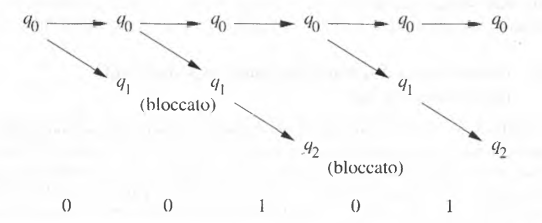
\includegraphics[scale=0.7]{img/nfa.png}
	\end{center}
	ovvero si parte dallo stato inziale, quando viene letto 0 si passa a $q_0$ e $q_1$, poi viene letto il secondo 0 quindi $q_0$ va nuovamente verso $q_0$ e $q_1$ mentre il primo $q_1$ muore non avendo transizioni su 0. Arriva poi l'1 quindi $q_0$ va solon verso $q_0$ e $q_1$ verso $q_2$ e sarebbe accettante ma l'input non è finito. Ora arriva 0 e $q_2$ si blocca mentre $q_0$ va sia in $q_0$ che in $q_1$. Arriva infine un 1 che manda $q_0$ in $q_0$ e $q_1$ in $q_2$ che è accettante e non avendo altri input si è dimostrata l'appartenenza della stringa al linguaggio
\end{example}
definisco quindi un NFA come una quintupla:
$A=(Q,\Sigma,\delta,q_0,F)$
con, a differenza dei DFA:
$\delta:Q\times F\to 2^Q$
Possiamo ora definire {$\delta$}, delta cappuccio che prende in ingresso uno stato e l'intera stringa $w$. Definisco ricorsivamente:
\begin{itemize}
	\item \textbf{caso base:} se $|w|=0$ ovvero se $W=\epsilon$ si ha:
	      $\hat{\delta}(q,\epsilon)=\{q\}$
	\item \textbf{caso passo:} se $|w|>0$, allora $W=xa$, $a\in\Sigma$ e $x\in\Sigma^*$. Posto $\hat{\delta}(q,x)=\{p_1,\cdots,p_k\}$ si ha:
	      $\hat{\delta}(q,w)=\cup \delta(p_i,a)$
\end{itemize}
%aggiungere esempio
Per il linguaggio $L$ accettato dall'automa si ha:
$L(A)=\{w\in \Sigma^*|\, \hat{\delta}(q_0,q)\cap F\neq \emptyset\}$
\begin{example}
	Automa per $L=\{x010y|\,x,y\in\{0,1\}^*\}$ ovvero tutte le stringhe con dentro la sequenza $010$:
	\begin{center}
		\begin{tikzpicture}[shorten >=1pt,node distance=2cm,on grid,auto]
			\node[state, initial] (q_0) {$q_{0}$};
			\node[state] (q_1) [right=of q_0] {$q_{1}$};
			\node[state] (q_2) [right=of q_1] {$q_{2}$};
			\node[state, accepting] (q_3) [right=of q_2] {$q_{3}$};
			\path[->]
			(q_0) edge  node {0} (q_1)
			edge [loop above] node {0,1} ()
			(q_1) edge  node {1} (q_2)
			(q_2) edge  node {0} (q_3)
			(q_3)     edge [loop above] node {0,1} ();
		\end{tikzpicture}
	\end{center}
\end{example}
Troviamo ora un algoritmo che trasformi un NFA in un DFA.
Dal penultimo esempio esempio ricavo:
\begin{center}
	\begin{tabular}{c|c|c}
		                     & 0             & 1             \\
		\hline
		$\emptyset$          & $\emptyset$   & $\emptyset$   \\
		\hline
		$\to \,\{q_0\}$      & $\{q_0,q_1\}$ & $\{q_0\}$     \\
		\hline
		$\,\{q_1\}$          & $\emptyset$   & $\{q_2\}$     \\
		\hline
		$*\,\{q_2\}$         & $\emptyset$   & $\emptyset$   \\
		\hline
		$\{q_0,q_1\}$        & $\{q_0,q_1\}$ & $\{q_0,q_2\}$ \\
		\hline
		$*\,\{q_0,q_2\}$     & $\{q_0,q_1\}$ & $\{q_0\}$     \\
		\hline
		$*\,\{q_1, q_2\}$    & $\emptyset$   & $\{q_2\}$     \\
		\hline
		$*\,\{q_0,q_1,q_2\}$ & $\{q_0,q_1\}$ & $\{q_0,q_2\}$
	\end{tabular}
\end{center}
ovvero:
\begin{center}
	\begin{tikzpicture}[shorten >=1pt,node distance=4cm,on grid,auto]
		\node[state, initial] (q_0) {$\{q_{0}\}$};
		\node[state] (q_1) [right=of q_0] {$\{q_{0}, q_1\}$};
		\node[state] (q_2) [right=of q_1] {$\{q_0,q_{2}\}$};
		\path[->]
		(q_0) edge  node {0} (q_1)
		edge [loop above] node {1} ()
		(q_1) edge  node {1} (q_2)
		edge [loop above] node {0} ()
		(q_2) edge [bend left =25]  node {0} (q_1)
		edge [bend left =45] node  {1} (q_0);
	\end{tikzpicture}
\end{center}
che è il DFA che si era anche prima ottenuto. Si hanno però dei sottoinsiemi mai raggiungibili. Si ha quindi:
\begin{center}
	\begin{tabular}{c|c|c}
		                 & 0             & 1             \\
		\hline
		$\to\,\{q_0\}$   & $\{q_0,q_1\}$ & $\{q_0\}$     \\
		\hline
		$\{q_0,q_1\}$    & $\{q_0,q_1\}$ & $\{q_0,q_2\}$ \\
		\hline
		$\,\{q_0, q_2\}$ & $\{q_0,q_1\}$ & $\{q_0\}$
	\end{tabular}
\end{center}
e definendo $\{q_0\}=a, \, \{q_0,q_1\}=b\,\,\, e\,\,\, \{q_0,q_2\}=c$ si avrà:
\begin{center}
	\begin{tikzpicture}[shorten >=1pt,node distance=2cm,on grid,auto]
		\node[state, initial] (q_0) {$a$};
		\node[state] (q_1) [right=of q_0] {$b$};
		\node[state, accepting] (q_2) [right=of q_1] {$c$};
		\path[->]
		(q_0) edge  node {0} (q_1)
		edge [loop above] node {1} ()
		(q_1) edge  node {1} (q_2)
		edge [loop above] node {0} ()
		(q_2) edge  [bend left =25] node {0} (q_1)
		edge [bend left = 50] node {1} (q_0);
	\end{tikzpicture}
\end{center}
Definiamo questo algoritmo che avrà:
\begin{itemize}
	\item come input un NFA $N=(Q_n,\Sigma,\delta_N,q_0,F_N)$
	\item come output un DFA $D=(Q_D,\Sigma,\delta_D,\{q_0\},F_D)$ tale che $L(D)=L(N)$
\end{itemize}
con:
\begin{itemize}
	\item $Q_D=2^{Q_N}$ (quindi se $Q_N=n$ si ha $|Q_D|=2^n$)
	\item $F_D=\{S\subseteq Q_n|\, S\cap F_N\neq \emptyset\}$
	\item $\forall S\subseteq Q_N$ e $ \forall a \in\Sigma$:
	      $\delta_D(S,a)=\cup \delta_n(p,a)$
	      per esempio:
	      $\delta_D(\{q_0,q_1,q_2\},0)=\delta_N(q_0,0)\cup \delta_N(q_1,0) \cup\delta_N(q_2,0) $
\end{itemize}
Si definisce l'$\epsilon-NFA$, l'automa astati finiti non deterministici con $\epsilon$ transizioni. Con la transizione $\epsilon$ posso saltare i nodi, ovvero avanza senza aggiungere caratteri
\begin{example}
	Si ha $ER=a^*b^*c^*$, che genera:
	$L=\{a^nb^mc^k|\,n,m,k\geq 0\}$
	si ha:
	\begin{center}
		\begin{tikzpicture}[shorten >=1pt,node distance=2cm,on grid,auto]
			\node[state, initial] (q_0) {$q_0$};
			\node[state] (q_1) [right=of q_0] {$q_1$};
			\node[state, accepting] (q_2) [right=of q_1] {$q_2$};
			\path[->]
			(q_0) edge  node {$\epsilon$} (q_1)
			edge [loop above] node {a} ()
			(q_1) edge  node {$\epsilon$} (q_2)
			edge [loop above] node {b} ()
			(q_2) edge  [loop above] node {c} ();
		\end{tikzpicture}
	\end{center}
	ovvero con $\epsilon$ posso per esempio generare quante $a$ voglio da $q_0$ e passare a $q_2$, uscendo senza generare altro
\end{example}
Si definisce la funzione $E\,CLOSE:Q\to 2^Q$, con $E\,CLOSE(q)$ insieme degli stati raggiungibili da $q$ tramite $\epsilon-mosse$. Nell'esempio precedente si avrebbe:
$E\,CLOSE(q_0)=\{q_0,q_1,q_2\}$
$E\,CLOSE(q_1)=\{q_1,q_2\}$
$E\,CLOSE(q_2)=\{q_2\}$
si ha inoltre che:
\begin{itemize}
	\item $E\,CLOSE 2^Q\to 2^Q\,\,\, P\subseteq Q$
	\item $E\,CLOSE(P)=\cup E\,CLOSE(p)$
	\item $E\,CLOSE(\emptyset)=\emptyset$
\end{itemize}
mettendo in tabella l'esempio precedente si ha:
\begin{center}
	\begin{tabular}{c|c|c|c}
		                        & a                 & b             & c           \\
		\hline
		$*\to\,\{q_0,q_1,q_2\}$ & $\{q_0,q_1,q_2\}$ & $\{q_1,q_2\}$ & $\{q_2\}$   \\
		\hline
		$*\{q_1,q_2\}$          & $\emptyset$       & $\{q_1,q_2\}$ & $\{q_2\}$   \\
		\hline
		$*\{q_2\}$              & $\emptyset$       & $\emptyset$   & $\{q_2\}$   \\
		\hline
		$\emptyset$             & $\emptyset$       & $\emptyset$   & $\emptyset$
	\end{tabular}
\end{center}
riscrivendo:
\begin{itemize}
	\item $a=\{q_0,q_1,q_2\}$
	\item $b=\{q_1,q_2\}$
	\item $c=\{q_2\}$
	\item $d=\emptyset$
\end{itemize}
ovvero:
$\delta_D(\{q_0,q_1,q_2\},a)=E\,CLOSE(\delta_N(q_0,a)\cup \delta_N(q_1,a)\cup \delta_N(q_2,a))$
$=E\,CLOSE(\{q_0\} \cup \emptyset\cup \emptyset)=E\,CLOSE(\{q_0\})$
$=E\,CLOSE	(q_0)=\{q_0,q_1,q_2\}$
e
$\delta_D(\{q_0,q_1,q_2\},B)=E\,CLOSE(\delta_N(q_0,b)\cup \delta_N(q_1,b)\cup \delta_N(q_2,b))$
$=E\,CLOSE(\emptyset \cup \{q_1\}\cup \emptyset)=E\,CLOSE(\{q_1\})$
$=E\,CLOSE	(q_1)=\{q_1,q_2\}$
e
$\delta_D(\{q_0,q_1,q_2\},c)=E\,CLOSE(\delta_N(q_0,c)\cup \delta_N(q_1,c)\cup \delta_N(q_2,c))$
$=E\,CLOSE(\emptyset \cup \emptyset\cup \{q_2\})=E\,CLOSE(\{q_1\})$
$=E\,CLOSE	(q_2)=\{q_2\}$

si ottiene quindi il seguente NFA:
\begin{center}
	\begin{tikzpicture}[shorten >=1pt,node distance=3cm,on grid,auto]
		\node[state, initial, accepting] (q_0) {$A$};
		\node[state, accepting] (q_1) [right=of q_0] {$B$};
		\node[state, accepting] (q_2) [below=of q_0] {$C$};
		\node[state] (q_3) [right=of q_2] {$D$};
		\path[->]
		(q_0) edge  node {b} (q_1)
		edge  node {c} (q_2)
		edge [loop above] node {a} ()
		(q_1) edge  node {c} (q_2)
		edge  node {a} (q_3)
		edge [loop above] node {b} ()
		(q_2) edge  node {a,b} (q_3)
		edge [loop below] node {c} ()
		(q_3) edge [loop below] node {a,b,c} ();
	\end{tikzpicture}
\end{center}
che diventa il seguente DFA:
\begin{center}
	\begin{tikzpicture}[shorten >=1pt,node distance=3cm,on grid,auto]
		\node[state, initial, accepting] (q_0) {$\{q_0,q_1,q_2\}$};
		\node[state, accepting] (q_1) [right=of q_0] {$\{q_1,q_2\}$};
		\node[state, accepting] (q_2) [below=of q_0] {$\{q_2\}$};
		\node[state] (q_3) [right=of q_2] {$q_E$};
		\path[->]
		(q_0) edge  node {b} (q_1)
		edge  node {c} (q_2)
		edge [loop above] node {a} ()
		(q_1) edge  node {c} (q_2)
		edge  node {a} (q_3)
		edge [loop above] node {b} ()
		(q_2) edge  node {a,b} (q_3)
		edge [loop below] node {c} ();
	\end{tikzpicture}
\end{center}

\subsubsection{esercizi}
\begin{example}
	automa DFA per $w=x010y,\,x,y\in\{0,1\}^*$ :
	la stringa più corta è 010
	\begin{center}
		\begin{tikzpicture}[shorten >=1pt,node distance=2cm,on grid,auto]
			\node[state, initial] (q_0) {$q_{0}$};
			\node[state] (q_1) [right=of q_0] {$q_{1}$};
			\node[state] (q_2) [right=of q_1] {$q_{2}$};
			\node[state, accepting] (q_3) [right=of q_2] {$q_{3}$};
			\path[->]
			(q_0) edge  node {0} (q_1)
			edge [loop above] node {1} ()
			(q_1) edge  node {1} (q_2)
			edge [loop above] node {0} ()
			(q_2) edge  node {0} (q_3)
			edge  [bend left = 45] node {1}(q_0)
			(q_3) edge [loop above] node {0,1} ();
		\end{tikzpicture}
	\end{center}
\end{example}
\begin{example}
	automa DFA per $a^{2k+1}b^{2h},\, h,k\geq 0$ :
	concatenazione di a dispari e b pari:
	\begin{center}
		\begin{tikzpicture}[shorten >=1pt,node distance=2cm,on grid,auto]
			\node[state, initial] (q_0) {$q_{0}$};
			\node[state, accepting] (q_1) [right=of q_0] {$q_{1}$};
			\node[state] (q_3) [right=of q_1] {$q_{3}$};
			\node[state] (q_2) [below= of q_1] {$q_{2}$};
			\node[state, accepting] (q_4) [right = of q_2] {$q_4$};
			\node[state] (q_5) [right=of q_4] {$q_E$};
			\path[->]
			(q_0) edge  node [bend left = 25] {a} (q_1)
			(q_1) edge [bend left = 25] node {a} (q_2)
			edge node [bend left= 25] {b} (q_3)
			(q_2) edge [bend left = 25] node [left] {a} (q_1)
			(q_3) edge [bend right = 25] node [left] {b} (q_4)
			(q_4) edge [bend right = 25] node [right] {b} (q_3)
			(q_2) edge  [bend right = 55] node [below] {b} (q_5)
			(q_3) edge  [bend left = 25] node {a} (q_5)
			(q_4) edge  [bend right = 25] node [below] {a} (q_5)
			(q_5) edge [loop right] node {a,b} ();
		\end{tikzpicture}
	\end{center}
\end{example}
\begin{example}
	cerco DFA per stringhe inizianti con a e finenti con b, con occorrenze di b singole o a coppie, nessuna regola per c.
	per esempio $abbcb$ è nel linguaggio
	\begin{center}
		\begin{tikzpicture}[shorten >=1pt,node distance=2cm,on grid,auto]
			\node[state, initial] (q_0) {$q_{0}$};
			\node[state] (q_1) [right=of q_0] {$q_{1}$};
			\node[state, accepting] (q_2) [right=of q_1] {$q_{2}$};
			\node[state, accepting] (q_3) [right= of q_3] {$q_{3}$};
			\node[state] (q_5) [below=of q_0] {$q_E$};
			\path[->]
			(q_0) edge  node [bend left = 25] {a} (q_1)
			edge  node [bend left = 25] {b,c} (q_5)
			(q_1) edge  node {b} (q_2)
			edge [loop] node {a,c} ()
			(q_2) edge [bend left = 25] node {a,c} (q_1)
			edge  node  {b} (q_3)
			(q_3) edge [bend left = 65] node [below] {b} (q_5)
			edge [bend left = 55] node {a,c} (q_1)
			(q_5) edge [loop left] node {a,b,c} ();
		\end{tikzpicture}
	\end{center}
\end{example}

\begin{example}
	cerco DFA per  stringhe di bit non contegano 000
	\begin{center}
		\begin{tikzpicture}[shorten >=1pt,node distance=2cm,on grid,auto]
			\node[state, initial, accepting] (q_0) {$q_0$};
			\node[state, accepting] (q_1) [right=of q_0]{$q_1$};
			\node[state, accepting] (q_2) [right=of q_1]{$q_2$};
			\node[state] (q_e) [right=of q_2]{$q_E$};
			\path[->]
			(q_0) edge  [bend left=25] node {0} (q_1)
			edge [loop] node {1} ()
			(q_1) edge node {0} (q_2)
			edge [bend left=25] node {1} (q_0)
			(q_2) edge node {0} (q_e)
			edge  [bend left=55] node{1} (q_0)
			(q_e) edge [loop ] node {0,1} ();
		\end{tikzpicture}
	\end{center}
\end{example}
\begin{example}
	cerco DFA per  stringhe di bit non contegano 000 almeno una volta
	\begin{center}
		\begin{tikzpicture}[shorten >=1pt,node distance=2cm,on grid,auto]
			\node[state, initial] (q_0) {$q_0$};
			\node[state] (q_1) [right=of q_0]{$q_1$};
			\node[state] (q_2) [right=of q_1]{$q_2$};
			\node[state, accepting] (q_e) [right=of q_2]{$q_E$};
			\path[->]
			(q_0) edge  [bend left=25] node {0} (q_1)
			edge [loop] node {1} ()
			(q_1) edge node {0} (q_2)
			edge [bend left=25] node {1} (q_0)
			(q_2) edge node {0} (q_e)
			edge  [bend left=55] node{1} (q_0)
			(q_e) edge [loop ] node {0,1} ();
		\end{tikzpicture}
	\end{center}
\end{example}
\begin{example}
	cerco DFA per  stringhe di bit che contengono 000 solo una volta
	\begin{center}
		\begin{tikzpicture}[shorten >=1pt,node distance=2cm,on grid,auto]
			\node[state, initial] (q_0) {$q_0$};
			\node[state] (q_1) [right=of q_0]{$q_1$};
			\node[state] (q_2) [right=of q_1]{$q_2$};
			\node[state, accepting] (q_3) [right=of q_2]{$q_3$};
			\node[state,accepting] (q_4) [below=of q_3] {$q_3$};
			\node[state] (q_5) [below=of q_4]{$q_5$};
			\node[state] (q_6) [below=of q_5]{$q_6$};
			\node[state] (q_e) [right=of q_3]{$q_E$};
			\path[->]
			(q_0) edge  [bend left=25] node {0} (q_1)
			edge [loop] node {1} ()
			(q_1) edge node {0} (q_2)
			edge [bend left=25] node {1} (q_0)
			(q_2) edge node {0} (q_3)
			edge  [bend left=45] node{1} (q_0)
			(q_3) edge node {0} (q_e)
			edge node {1} (q_4)
			(q_4) edge [bend left=25] node {0} (q_5)
			edge [loop right] node {1} ()
			(q_5) edge [bend left=25] node {1} (q_4)
			edge node {0} (q_6)
			(q_6) edge [bend right=25] node {0} (q_e)
			edge [bend left=55] node {0} (q_4)
			(q_e) edge [loop ] node {0,1} ();
		\end{tikzpicture}
	\end{center}
\end{example}

\begin{example}
	Trasformare il seguente NFA in un DFA:
	\begin{center}
		\begin{tikzpicture}[shorten >=1pt,node distance=3cm,on grid,auto]
			\node[state, initial, accepting] (q_0) {$q_0$};
			\node[state, accepting] (q_1) [above right=of q_0] {$q_1$};
			\node[state] (q_2) [below right =of q_0] {$q_2$};
			\node[state] (q_3) [below right=of q_1] {$q_3$};
			\path[->]
			(q_0) edge  [bend left=25] node {a} (q_1)
			edge  [bend right=25] node [below] {b} (q_2)
			(q_1) edge  [bend left=25] node {a} (q_2)
			edge [loop ] node {a} ()
			(q_2) edge  [bend left=25] node {b} (q_1)
			edge  [bend right=15] node [below] {b} (q_3)
			(q_3) edge   node [above] {a} (q_1)
			edge  [bend right=15] node [above] {a} (q_2);
		\end{tikzpicture}
	\end{center}
	abbiamo quindi:
	$\delta_D(\{q_0\},a)=\delta_N(q_0,a)=\{q_1,q_2\}$
	$\delta_D(\{q_0\},b)=\delta_N(q_1,b)=\emptyset$
	$\delta_D(\{q_1,q_2\},a)=\delta_N(q_1,a)\cup \delta_N(q_2,a)=\{q_1,q_2\}cup \emptyset=\{q_1,q_2\}$
	$\delta_D(\{q_1,q_2\},b)=\delta_N(q_1,b)\cup \delta_N(q_2,b)=\emptyset\cup \{q_1,q_3\}=\{q_1,q_3\}$
	$\cdots$
	ottengo quindi:
	\begin{center}
		\begin{tabular}{c|c|c}
			DFA             & a             & b             \\
			\hline
			$*\to\,\{q_0\}$ & $\{q_1,q_2\}$ & $\emptyset$   \\
			\hline
			$*\{q_1,q_2\}$  & $\{q_1,q_2\}$ & $\{q_1,q_3\}$ \\
			\hline
			$\emptyset$     & $\emptyset$   & $\emptyset$   \\
			\hline
			$*\{q_1,q_3\}$  & $\{q_1,q_2\}$ & $\emptyset$
		\end{tabular}
	\end{center}
	Posso ora rinominare:
	\begin{itemize}
		\item $A=\{q_0\}$
		\item $B=\{q_1,q_2\}$
		\item $C=\emptyset$
		\item $D=\{q_1,q_3\}$
	\end{itemize}

	ottengo quindi il seguente DFA:
	\begin{center}
		\begin{tikzpicture}[shorten >=1pt,node distance=3cm,on grid,auto]
			\node[state, initial, accepting] (q_0) {$A$};
			\node[state, accepting] (q_1) [right=of q_0] {$B$};
			\node[state] (q_2) [below=of q_0] {$C$};
			\node[state,accepting] (q_3) [right=of q_2] {$D$};
			\path[->]
			(q_0) edge  node {a} (q_1)
			edge  node {b} (q_2)
			(q_1) edge  [bend left=25] node {b} (q_3)
			edge  [loop] node {a} ()
			(q_2) edge  [loop below] node {a,b} ()
			(q_3) edge  [bend left=25] node {a} (q_1)
			edge  node  {a} (q_2);
		\end{tikzpicture}
	\end{center}
\end{example}
\begin{example}
	Trasformare il seguente $\epsilon$-NFA in un DFA:
	\begin{center}
		\begin{tikzpicture}[shorten >=1pt,node distance=3cm,on grid,auto]
			\node[state, initial] (q_0) {$p$};
			\node[state] (q_1) [right=of q_0] {$q$};
			\node[state, accepting] (q_2) [below right =of q_0] {$r$};
			\path[->]
			(q_0) edge  [bend left=25] node [left] {c} (q_2)
			edge  [bend right=25] node {b} (q_1)
			edge [loop ] node {a} ()
			(q_1) edge  [bend right=25] node {$\epsilon$} (q_0)
			edge  [bend right=25] node [left] {b} (q_2)
			edge  [loop ] node {a} ()
			(q_2) edge  [bend left=25] node {c} (q_0)
			edge  [bend right=25] node [right] {$\epsilon$} (q_1)
			edge  [loop below] node {a} ();
		\end{tikzpicture}
	\end{center}
	vediamo le ECLOSE:
	$ECLOSE(p)=\{p\}$
	$ECLOSE(q)=\{p,q\}$
	$ECLOSE(r)=\{p,q,r\}$
	si ottiene quindi:
	\begin{center}
		\begin{tabular}{c|c|c|c}
			             & a           & b           & c           \\
			\hline
			$to\,\{p\}$  & $\{p\}$     & $\{p,q\}$   & $\{p,q,r\}$ \\
			\hline
			$\{p,q\}$    & $\{p,q\}$   & $\{p,q,r\}$ & $\{p,q,r\}$ \\
			\hline
			$*\{p,q,r\}$ & $\{p,q,r\}$ & $\{p,q,r\}$ & $\{p,q,r\}$
		\end{tabular}
	\end{center}
	infatti, per esempio:
	$\delta_D(\{p\}, a)= ECLOSE (\delta_(p,a))=ECLOSE (\{p\})=ECLOSE (p)=\{p\}$
	$\delta_D(\{p,q\}, a)= ECLOSE (\delta_N(p,a)\cup \delta_N(q,a))=$
	$ECLOSE (\{p\}\cup \{q\})=ECLOSE(P)\cup ECLOSE(q)=\{p\}\cup\{p,q\}=\{p,q\}$
	$\cdots$
	si hanno quindi le seguenti rinominazioni:
	\begin{itemize}
		\item $A=\{p\}$
		\item $b=\{p,q\}$
		\item $C=\{p,q,r\}$
	\end{itemize}
	ovvero:
	\begin{center}
		\begin{tikzpicture}[shorten >=1pt,node distance=3cm,on grid,auto]
			\node[state, initial] (q_0) {$A$};
			\node[state] (q_1) [right=of q_0] {$B$};
			\node[state, accepting] (q_2) [below=of q_0] {$C$};
			\path[->]
			(q_0) edge  node {b} (q_1)
			edge  node {c} (q_2)
			edge  [loop] node {a} ()
			(q_1) edge  node {b,c} (q_2)
			edge  [loop] node {a} ()
			(q_2) edge  [loop below] node {a,b,c} ();
		\end{tikzpicture}
	\end{center}
\end{example}

torniamo a dare bene qualche definizione per {$\delta$} in un DFA:
\begin{center}
	$\delta:Q\times \Sigma^* \to Q$
\end{center}
con: $q\in Q,\,\,\, w\in \Sigma^*\,\,\,e\,\,\,${$\delta$}$(p,w)=q$
\begin{itemize}
	\item
	      \textbf{caso base:} $w=\epsilon\to |w|=0\to${$\delta$}$(q,\epsilon)=q$

	      \textbf{caso passo:} $|w|\neq0\to w=ax$ con $a\in \Sigma,x\in \Sigma^*$:
	      {$\delta$}$(q,w)=${$\delta$}$(q,ax)=${$\delta$} $(\delta(q,a),x)$
	\item
	      \textbf{caso base:} $w=\epsilon\to |w|=0\to \delta(q,w)=\delta(q,\epsilon)=q$

	      \textbf{caso passo:} $|w|\neq0\to w=xa$ con $a\in \Sigma,x\in \Sigma^*$:
	      {$\delta$}$(q,w)=${$\delta$}$(q,xa)=${$\delta$} $(\delta(q,x),a)$
\end{itemize}
in un NFA si ha:
\begin{itemize}
	\item \textbf{caso base:}  {$\delta$}$(q,\epsilon=\{q\},\,\,\forall q\in Q$
	\item \textbf{caso passo:} posto $w=ax$ e {$\delta$}$(q,a)=\{p_1,\cdots,p_n$ allora {$\delta$}$(q,w)=\cup${$\delta$}$(p_i, x)0\{r_1,\cdots,r_n\}$.
	      {$\delta$}$(q,a)=p$
	      {$\delta$}$(q,w)=$ {$\delta$}$(q,xa)=$ {$\delta$}$(p,x)=r$
\end{itemize}
oppure:
\begin{itemize}
	\item \textbf{caso base:}  {$\delta$}$(q,\epsilon)=\{q\},\,\forall q\in Q$
	\item \textbf{caso passo:} posto $w=xa$ si ha  {$\delta$}$(q,q)=$ {$\delta$}$(q,xa)=\cup \delta(p,a)$ con  {$\delta$}$(q,x)=\{p_1,\cdots,p_n\}$
\end{itemize}
Se ho un NFA $N=(Q_N, \Sigma, \delta_N, q_{0_N}, F_N)$ con $\delta_N: Q\times\Sigma^*\to 2^{Q_N}$ che accetta un lingiaggio $L$ posso ottenere un DFA $D=(Q_D, \Sigma, \delta_D, q_{0_D}, F_D)$ equivalente con $Q_D=2^{Q_N}$  e $q_{0_D}=\{q_{0_N}\}$ che accetta L.
$\forall S\subseteq Q_N$ e $\forall a\in \Sigma$ si ha:
$F_D=\{S\subseteq Q_N\,|\, S\cap F_n\neq \emptyset\}$
con $\delta_D(S,a)=\cup \delta_N(p,a)$
Si ha che:
$|Q_D|=|2^{Q_N}|=2^{|Q_N|}$
partiamo con un esempio:
\begin{center}
	\begin{tikzpicture}[shorten >=1pt,node distance=2cm,on grid,auto]
		gin{tikzpicture}[shorten >=1pt,node distance=2cm,on grid,auto]
		\node[state,initial] (q_0)   {$q_0$};
		\node[state] (q_1) [right=of q_0] {$q_1$};
		\node[state] (q_2) [right=of q_1] {$\cdots$};
		\node[state] (q_3) [right=of q_2] {$q_{n-1}$};
		\node[state, accepting] (q_4) [right=of q_3] {$q_n$};
		\path[->]
		(q_0) edge  node {1} (q_1)
		edge [loop above] node {0,1} ()
		(q_1) edge  node {0,1} (q_2)
		(q_2) edge node {0,1} (q_3)
		(q_3) edge node {0,1} (q_4);
	\end{tikzpicture}
\end{center}
che definisce un $L\subseteq\{0,1\}^*$ tale che $w\in L$ sse n-simo elemento della fine è 1. Si ha:
$|Q_N|=n+1\to |Q_D|=2^n$
Si ha che dato un $\epsilon$-NFA $E=(Q_E, \Sigma, \delta_E, q_{0_E}, F_E)$ che riconosce $L$ in un NFA $N=(Q_N, \Sigma, \delta_N, q_{0_N}, F_N)$ equivalenti con $Q_N=2^{Q_E}$ stati in $Q_E$ $\epsilon$-close: \textit{ECLOSE(S)=S} e $q_N=ECLOSE(q_E)$:
$F_N\{S\in Q_F,\,\, S\subseteq Q_E | S\cap F_E\neq \emptyset\}$
quindi:
$\forall a\in \Sigma \text{ e } \forall S=\{p_1,\cdots,p_k\}, \forall S\in Q_F \text{ e } Q_E$
$\delta_F(S,a) \text{ si ottiene }\cup \delta_E(p_i,a)=\{r_1,\cdots, r_n\}$
$\delta_N(S,a)=ECLOSE(\{r_1, \cdots, r_n\})$

\begin{Exercise}\label{exe:no-101-er}
Costruire un'espressione regolare per il linguaggio $L\in\Sigma_{B}$ delle parole che non contengono la sottostringa \texttt{101}.
\end{Exercise}

\begin{Answer}
Una possibilità, che verrà formalizzata in \Cref{sec:da-DFA-a-ER} consiste nel partire dal DFA che riconosce il
linguaggio e sintetizzare l'espressione regolare a partire dall'automa.

Per ottenere un'ER semplice è invece preferibile ragionare sulla definizione di linguaggio da esprimere.
Una definizione equivalente è l'insieme delle parole in cui ogni occorrenza del carattere \texttt{1} è seguita da un
altro \texttt{1}, oppure da \texttt{00}, oppure ancora tale \texttt{1} è uno degli ultimi due caratteri della parola (in
questo caso, non potrà essere il carattere iniziale di una sottostringa \texttt{101})
Questa formulazione si presta maggiormente a disegnare un'espressione regolare.
Infatti, una riscrittura diretta di quanto descritto sopra, tenendo presente che un numero arbitrari di \texttt{0}
potrebbe precedere il primo \texttt{1} e seguire ogni \texttt{0}, diventa
$$\texttt{0}^{*}(\texttt{100}\texttt{0}^{*})^{*} (\texttt{10} |\texttt{1} | \epsilon)$$ che può essere ulteriormente
semplificata in
$$\texttt{0}^{*}(\texttt{100}\texttt{0}^{*})^{*} \texttt{1}^{*} \texttt{0}^{*}.$$
\end{Answer}



\begin{Exercise}\label{exe:no-diff2-er}
Costruire un'espressione regolare per il linguaggio $L\in\Sigma_{B}$ delle parole che soddisfano le due seguenti
condizioni:
\begin{enumerate}
\item hanno lo stesso numero di \zero e \uno
\item in ogni prefisso il numero di \zero e \uno differisce al massimo di $1$.
\end{enumerate}
Sono quindi parole del linguaggio $\epsilon$, \zero\uno, \texttt{10}, \texttt{101010}, \texttt{0101}.
Non sono parole del linguaggio \texttt{1100}.
\end{Exercise}

\begin{Exercise}\label{exe:3x3}
Costruire un'espressione regolare per il linguaggio $L\in\Sigma_{B}$ delle parole con un numero di \zero multiplo di $3$ e
un numero di \uno multiplo di $3$.
\end{Exercise}


\section{Da DFA a espressioni regolari}
\label{sec:da-DFA-a-ER}

\begin{itemize}
	\item \textbf{caso base}:
	      \begin{enumerate}
		      \item se $R=\epsilon$ ovvero $L(R)=\{\epsilon\}$ allora:
		            \begin{center}
			            \begin{tikzpicture}[shorten >=1pt,node distance=2cm,on grid,auto]
				            \node[state,initial] (q_0)   {$q_0$};
				            \node[state, accepting] (q_1) [right=of q_0] {$q_1$};
				            \path[->]
				            (q_0) edge node {$\epsilon$} (q_1);
			            \end{tikzpicture}
		            \end{center}
		      \item se $R=\emptyset$ ovvero $L(R)=\emptyset$ allora:
		            \begin{center}
			            \begin{tikzpicture}[shorten >=1pt,node distance=2cm,on grid,auto]
				            \node[state,initial] (q_0)   {$q_0$};
				            \node[state, accepting] (q_1) [right=of q_0] {$q_1$}; ;
			            \end{tikzpicture}
		            \end{center}
		      \item se $R=a$ ovvero $L(R)=\{a\}$ allora:
		            \begin{center}
			            \begin{tikzpicture}[shorten >=1pt,node distance=2cm,on grid,auto]
				            \node[state,initial] (q_0)   {$q_0$};
				            \node[state, accepting] (q_1) [right=of q_0] {$q_1$};
				            \path[->]
				            (q_0) edge node {a} (q_1);
			            \end{tikzpicture}
		            \end{center}
	      \end{enumerate}
	\item \textbf{caso passo:}
	      \begin{enumerate}
		      \item se $R=S+T$ quindi $L(R)=L(S)+L(T)$ allora:
		            \begin{center}
			            \begin{tikzpicture}[shorten >=1pt,node distance=2cm,on grid,auto]
				            \node[state,initial] (q_0)   {$q_0$};
				            \node[state] (q_1) [above right =of q_0] {$q_1$};
				            \node[state] (q_2) [below right =of q_0] {$q_2$};
				            \node[draw=none,fill=none] (Q_E) [right = of q_1] {$S$};
				            \node[draw=none,fill=none] (Q_F) [right = of q_2] {$S$};
				            \node[state] (q_3) [right=of Q_E] {$q_3$};
				            \node[state] (q_4) [right=of Q_F] {$q_4$};
				            \node[state, accepting] (q_5) [below right =of q_3] {$q_5$};
				            \path[->]
				            (q_0) edge node {$\epsilon$} (q_1)
				            (q_0) edge node {$\epsilon$} (q_2)
				            (q_3) edge node {$\epsilon$} (q_5)
				            (q_4) edge node {$\epsilon$} (q_5);
			            \end{tikzpicture}
		            \end{center}
		      \item se $R=ST$ quindi $L(R)=L(S)L(T)$:
		            \begin{center}
			            \begin{tikzpicture}[shorten >=1pt,node distance=2cm,on grid,auto]
				            \node[state,initial] (q_0)   {$q_0$};
				            \node[draw=none,fill=none] (Q_E) [right = of q_0] {$S$};
				            \node[state] (q_1) [ right =of Q_E] {$q_1$};
				            \node[state] (q_2) [right =of q_1] {$q_2$};
				            \node[draw=none,fill=none] (Q_F) [right = of q_2] {$T$};
				            \node[state] (q_3) [right=of Q_F] {$q_3$};
				            \node[draw=none,fill=none] (Q_G) [right = of q_3] {};
				            \path[->]
				            (q_1) edge node {$\epsilon$} (q_2)
				            (q_3) edge node {} (Q_G);
			            \end{tikzpicture}
		            \end{center}
		      \item se $R=S^*$ quindi $L(R)=(L(S))^*$:
		            \begin{center}
			            \begin{tikzpicture}[shorten >=1pt,node distance=2cm,on grid,auto]
				            \node[state,initial] (q_0)   {$q_0$};
				            \node[state] (q_1) [ right =of Q_E] {$q_1$};
				            \node[draw=none,fill=none] (Q_F) [right = of q_1] {$S$};
				            \node[state] (q_2) [right =of Q_F] {$q_2$};
				            \node[state] (q_3) [right=of q_2] {$q_3$};
				            \path[->]
				            (q_0) edge node {$\epsilon$} (q_1)
				            (q_2) edge [bend right = 35]  node {$\epsilon$} (q_1)
				            (q_0) edge [bend right = 25] node  {$\epsilon$} (q_3)
				            (q_2) edge node {$\epsilon$} (q_3);
			            \end{tikzpicture}
		            \end{center}
	      \end{enumerate}
\end{itemize}




\begin{example}
	creo E-NFA per
	$ER=(0+1)^*1(0+1)$
	si ha che per 0+1:
	\begin{center}
		\begin{tikzpicture}[shorten >=1pt,node distance=2cm,on grid,auto]
			\node[state,initial] (q_0)   {$q_0$};
			\node[state] (q_1) [above right =of q_0] {$q_1$};
			\node[state] (q_2) [below right =of q_0] {$q_2$};
			\node[state] (q_3) [right=of q_1] {$q_3$};
			\node[state] (q_4) [right=of q_2] {$q_4$};
			\node[state] (q_5) [below right =of q_3] {$q_5$};
			\path[->]
			(q_0) edge node {$\epsilon$} (q_1)
			(q_0) edge node {$\epsilon$} (q_2)
			(q_1) edge node {$0$} (q_3)
			(q_2) edge node {$1$} (q_4)
			(q_3) edge node {$\epsilon$} (q_5)
			(q_4) edge node {$\epsilon$} (q_5);
		\end{tikzpicture}
	\end{center}
	da qui ottengo $(0+1)^*$
	\begin{center}
		\begin{tikzpicture}[shorten >=1pt,node distance=2cm,on grid,auto]
			\node[state, initial] (q_i)   {$q_i$};
			\node[state] (q_0) [right of = q_i]  {$q_0$};
			\node[state] (q_1) [above right =of q_0] {$q_1$};
			\node[state] (q_2) [below right =of q_0] {$q_2$};
			\node[state] (q_3) [right=of q_1] {$q_3$};
			\node[state] (q_4) [right=of q_2] {$q_4$};
			\node[state] (q_5) [below right =of q_3] {$q_5$};
			\node[state, accepting] [right of =q_5] (q_f)   {$q_f$};
			\path[->]
			(q_i) edge node {$\epsilon$} (q_0)
			(q_i) edge [bend right =65] node {$\epsilon$} (q_f)
			(q_0) edge node {$\epsilon$} (q_1)
			(q_0) edge node {$\epsilon$} (q_2)
			(q_1) edge node {$0$} (q_3)
			(q_5) edge  [bend right =100] node [above] {$\epsilon$} (q_0)
			(q_2) edge node {$1$} (q_4)
			(q_3) edge node {$\epsilon$} (q_5)
			(q_5) edge node {$\epsilon$} (q_f)
			(q_4) edge node {$\epsilon$} (q_5);
		\end{tikzpicture}
	\end{center}
	unisco e aggiungo uno nel mezzo:
	\begin{center}
		\begin{tikzpicture}[shorten >=1pt,node distance=1.4cm,on grid,auto]
			\node[state, initial] (q_i)   {$q_i$};
			\node[state] (q_0) [right of = q_i]  {$q_0$};
			\node[state] (q_1) [above right =of q_0] {$q_1$};
			\node[state] (q_2) [below right =of q_0] {$q_2$};
			\node[state] (q_3) [right=of q_1] {$q_3$};
			\node[state] (q_4) [right=of q_2] {$q_4$};
			\node[state] (q_5) [below right =of q_3] {$q_5$};
			\node[state] (q_f) [below right =of q_5] {$q_f$};

			\node[state] (q_m) [right of = q_f]  {$q_m$};
			\node[state] (q_n) [right =of q_m] {$q_n$};

			\node[state] (q_6) [right of = q_n]  {$q_6$};
			\node[state] (q_7) [above right =of q_6] {$q_7$};
			\node[state] (q_8) [below right =of q_6] {$q_8$};
			\node[state] (q_9) [right=of q_7] {$q_9$};
			\node[state] (q_a) [right=of q_8] {$q_a$};
			\node[state] (q_b) [below right =of q_9] {$q_b$};
			\path[->]
			(q_i) edge node {$\epsilon$} (q_0)
			(q_i) edge [bend right =65] node {$\epsilon$} (q_f)
			(q_0) edge node {$\epsilon$} (q_1)
			(q_0) edge node {$\epsilon$} (q_2)
			(q_1) edge node {$0$} (q_3)
			(q_5) edge  [bend right =100] node [above] {$\epsilon$} (q_0)
			(q_2) edge node {$1$} (q_4)
			(q_3) edge node {$\epsilon$} (q_5)
			(q_5) edge node {$\epsilon$} (q_f)
			(q_4) edge node {$\epsilon$} (q_5)
			(q_f) edge node  {$\epsilon$} (q_m)
			(q_m) edge node  {$1$} (q_n)
			(q_n) edge node  {$\epsilon$} (q_6)
			(q_6) edge node {$\epsilon$} (q_7)
			(q_6) edge node {$\epsilon$} (q_8)
			(q_6) edge node {$0$} (q_8)
			(q_7) edge node {$1$} (q_9)
			(q_8) edge node {$\epsilon$} (q_a)
			(q_a) edge node {$\epsilon$} (q_b)
			(q_9) edge node {$\epsilon$} (q_b);
		\end{tikzpicture}
	\end{center}
\end{example}
Vediamo ora l'algoritmo che trasforma DFA in una ER. Questo algoritmo permette di verificare quale linguaggio è accettato o meno dall'automa:
dato DFA $A=(Q,\Sigma, \delta, q_0,F)$ con $Q$ e $F$ stati non finali e $Q$, $F$, $q_0$ che sono i primi stati da eliminare. L'algoritmo procede per eliminazioni successive. Si costruisce quindi l'automa $B$ che ha solo $q_0$ e $F=\{q_1,\cdots,q_k\}$. Scrivo quindi $K$ espressioni regolari considerando solo $q_0$ e il k-esimo stato finale eliminando pian piano gli altri stati. Alla fine ottengo le varie espressioni regolari da unire:
$E=E1+E2+\cdots+Ek$
vediamo ora come eliminare uno stato. Partiamo dal seguente automa:
\begin{center}
	\begin{tikzpicture}[shorten >=1pt,node distance=4cm,on grid,auto]
		\node[state] (q_1)   {$q_1$};
		\node[state] (s) [below right =of q_1] {$s$};
		\node[state] (q_k) [below left =of s] {$q_k$};
		\node[state] (p_1) [above right=of s] {$p_1$};
		\node[state] (p_m) [below right =of s] {$p_m$};
		\path[->]
		(q_1) edge node {$Q_1$} (s)
		(q_1) edge [bend left =50] node {$R_{11}$} (p_1)
		(q_1) edge [bend left =100] node {$R_{1m}$} (p_m)
		(s)   edge node {$p_1$} (p_1)
		(s)   edge node {$p_m$} (p_m)
		(s)   edge [loop above] node {$S$} ()
		(q_k) edge node {$Q_k$} (s)
		(q_k) edge [bend right =50] node {$R_{k1}$} (p_1)
		(q_k) edge [bend right =100] node {$R_{km}$} (p_m);
	\end{tikzpicture}
\end{center}

ed elimino $s$:
\begin{center}
	\begin{tikzpicture}[shorten >=1pt,node distance=4cm,on grid,auto]
		\node[state] (q_1)   {$q_1$};
		\node[state] (q_k) [below =of q_1] {$q_k$};
		\node[state] (p_1) [right=of q_1] {$p_1$};
		\node[state] (p_m) [below  =of p_1] {$p_m$};
		\path[->]
		(q_1) edge node {$R_{11}+Q_1S^{*}P_1$} (p_1)
		(q_1) edge node [right]{$R_{1m}+Q_1S^{*}P_m$} (p_m)
		(q_k) edge node [left]{$R_{k1}+Q_kS^{*}P_1$} (p_1)
		(q_k) edge node {$R_{km}+Q_kS^{*}P_m$} (p_m);
	\end{tikzpicture}
\end{center}
quindi quando si ha uno stato iniziale $q_0$ e uno finale $q_1$:
\begin{itemize}
	\item se $q_0\neq q_1$:
	      \begin{center}
		      \begin{tikzpicture}[shorten >=1pt,node distance=3cm,on grid,auto]
			      \node[state, initial] (q_0)   {$q_1$};
			      \node[state, accepting] (q_1) [right=of q_1] {$q_k$};
			      \path[->]
			      (q_0) edge [bend left =25]node {$S$} (q_1)
			      (q_1) edge [bend left =25]node {$T$} (q_0)
			      (q_0)   edge [loop above] node {$R$} ()
			      (q_1)   edge [loop above] node {$U$} ();
		      \end{tikzpicture}
	      \end{center}
	      rappresenta:
	      $E_i=(R+SU^{*}T)^{*}SU^{*}$
	\item se $q_0=q$:
	      \begin{center}
		      \begin{tikzpicture}[shorten >=1pt,node distance=3cm,on grid,auto]
			      \node[state, initial, accepting] (q_0)   {$q_1$};
			      \path[->]
			      (q_0)   edge [loop above] node {$R$} ();
		      \end{tikzpicture}
	      \end{center}
	      rappresenta:
	      $E_i=R^{*}$
\end{itemize}

\begin{example}
	passo dall'automa a l'espressione regolare:
	\begin{center}
		\begin{tikzpicture}[shorten >=1pt,node distance=2cm,on grid,auto]
			\node[state, initial] (q_0) {$A$};
			\node[state] (q_1) [right=of q_0] {$B$};
			\node[state, accepting] (q_2) [right=of q_1] {$C$};
			\node[state, accepting] (q_3) [right=of q_2] {$D$};
			\path[->]
			(q_0) edge  node {1} (q_1)
			edge [loop above] node {0,1} ()
			(q_1) edge  node {0,1} (q_2)
			(q_2) edge  node {0,1} (q_3);
		\end{tikzpicture}
	\end{center}
	questo automa accetta le stringhe binarie con un uno in penultima o terzultima posizione.
	Rietichetto con le ER:
	\begin{center}
		\begin{tikzpicture}[shorten >=1pt,node distance=2cm,on grid,auto]
			\node[state, initial] (q_0) {$A$};
			\node[state] (q_1) [right=of q_0] {$B$};
			\node[state, accepting] (q_2) [right=of q_1] {$C$};
			\node[state, accepting] (q_3) [right=of q_2] {$D$};
			\path[->]
			(q_0) edge  node {1} (q_1)
			edge [loop above] node {0+1} ()
			(q_1) edge  node {0+1} (q_2)
			(q_2) edge  node {0+1} (q_3);
		\end{tikzpicture}
	\end{center}
	elimino B che non è iniziale o finale . Il predecessore di B è A e il successore è C. Si ha quindi:
	$A\to B:1$
	$B\to C:0+1$
	e non ho loop in B ($\emptyset$) e nessun arco tra A e C ($R_{a,c}=\emptyset$). Quindi:
	$R_{A,C}^{'}=\emptyset+1\emptyset^*(0+1)=1(0+1)$
	ovvero:
	\begin{center}
		\begin{tikzpicture}[shorten >=1pt,node distance=3cm,on grid,auto]
			\node[state, initial] (q_0) {$A$};
			\node[state, accepting] (q_2) [right=of q_0] {$C$};
			\node[state, accepting] (q_3) [right=of q_2] {$D$};
			\path[->]
			(q_0) edge  node {1(0+1)} (q_2)
			edge [loop above] node {0+1} ()
			(q_2) edge  node {0+1} (q_3);
		\end{tikzpicture}
	\end{center}
	Ho ora solo stati iniziali e finali, quindi $E=E_1+E_2$.
	Trovo $E1$, elimino quindi C. Si ha:
	$A\to C:1(0+1)$
	$C\to D:0+1$
	e non ho loop in B ($\emptyset$) e nessun arco tra A e D($R_{A,D}=\emptyset$), ovvero:
	$R_{A,D}=\emptyset+1(0+1)\emptyset^*(0+1)=1(0+1)(0+1)$
	che è:
	\begin{center}
		\begin{tikzpicture}[shorten >=1pt,node distance=4cm,on grid,auto]
			\node[state, initial] (q_0) {$A$};
			\node[state, accepting] (q_3) [right=of q_0] {$D$};
			\path[->]
			(q_0) edge  node {1(0+1)(0+1)} (q_3)
			edge [loop above] node {0+1} ();
		\end{tikzpicture}
	\end{center}
	quindi:
	$E_1=((0+1)+1(0+1)(0+1)\emptyset^*\emptyset)^*1(0+1)(0+1)\emptyset^*=(0+1)^*1(0+1)(0+1)$
	ottengo $E2$ eliminando D che non ha successori, quindi:
	$E_2=(0+1)^*1(0+1)$
	e quindi infine:
	$E=E_1+E_2=(0+1)^*1(0+1)(0+1)+(0+1)^*1(0+1)=(0+1)^*1(0+1)(\epsilon+0+1)$
\end{example}
\begin{example}
	\begin{center}
		\begin{tikzpicture}[shorten >=1pt,node distance=3cm,on grid,auto]
			\node[state, initial, accepting] (q_0) {$p$};
			\node[state] (q_1) [right =of q_0] {$s$};
			\node[state] (q_2) [right=of q_1] {$r$};
			\node[state] (q_3) [below=of q_1] {$q$};
			\path[->]
			(q_0) edge  node {0} (q_1)
			edge [loop above] node {1} ()
			(q_1) edge [bend left = 25] node {0} (q_3)
			(q_1) edge  node {1} (q_2)
			(q_2) edge  [bend left = 25] node {1} (q_3)
			edge [loop above] node {0} ()
			(q_3) edge  [bend left = 25] node {1} (q_1)
			(q_3) edge  [bend left = 25] node {0} (q_0);
		\end{tikzpicture}
	\end{center}
	rimuovo $r$:
	$s\to r:1$
	$r\to q:1$
	$loop:0$
	$R_{s,q}=0$
	Si ottiene quindi:
	$R^{'}_{s,q}=0+10^*1$
	ovvero:
	\begin{center}
		\begin{tikzpicture}[shorten >=1pt,node distance=3cm,on grid,auto]
			\node[state, initial, accepting] (q_0) {$p$};
			\node[state] (q_1) [right =of q_0] {$s$};
			\node[state] (q_3) [below=of q_1] {$q$};
			\path[->]
			(q_0) edge  node {0} (q_1)
			edge [loop above] node {1} ()
			(q_1) edge [bend left = 25] node {$0+10^*1$} (q_3)
			(q_3) edge  [bend left = 25] node {1} (q_1)
			(q_3) edge  [bend left = 25] node {0} (q_0);
		\end{tikzpicture}
	\end{center}
	elimino ora $s$, che ha due predecessori, $p$ e $q$, quindi:
	$p\to s:0$
	$q\to s:1$
	$s\to q:0+10^*1$
	non ha loop e non ha archi diretti tra $p$ e $q$ ($R_{p,q}=\emptyset$). Si ottengono quindi:
	$R_{p,q}=\emptyset+0\emptyset^*(0+10^*1)=0(0+10^*1)$
	$R_{q,q}=\emptyset+10^*(0+10^*1)=1(0+10^*1)$
	\begin{center}
		\begin{tikzpicture}[shorten >=1pt,node distance=4cm,on grid,auto]
			\node[state, initial, accepting] (q_0) {$p$};
			\node[state] (q_3) [right=of q_0] {$q$};
			\path[->]
			(q_0) edge [bend left = 25] node {$0(0+10^*1)$} (q_3)
			edge [loop above] node {1} ()
			(q_3) edge  [bend left = 25] node {0} (q_0)
			edge [loop above] node {$1(0+10^*1)$} ();
		\end{tikzpicture}
	\end{center}
	elimino ora $q$ che ha $p$ sia come predecessore che come successore:
	$p\to q: 0(0+10^*1)$
	$q\to p:0$
	$loop: 1(0+10^*1)$
	$R_{p,p}:1$
	ottenendo:
	$R^{'}_{p,p}=1+0(0+10^*1)(1(0+10^*1))^*0=1+(00+010^*1)(10+110^*1)^*0$

	ovvero:

	\begin{center}
		\begin{tikzpicture}[shorten >=1pt,node distance=4cm,on grid,auto]
			\node[state, initial, accepting] (q_0) {$p$};
			\path[->]
			(q_0)   edge [loop above] node {$1+(00+010^*1)(10+110^*1)^*0$} ();
		\end{tikzpicture}
	\end{center}
	Essendo $p$ sia iniziale che finale si ha:
	$E=(1+(00+010^*1)(10+110^*1)^*0)^*$
\end{example}

\section{Da espressioni regolari a ε-NFA}
\label{sec:da-ER-a-eNFA}

\begin{Exercise}\label{exe:er-nfa-1}
Costruire l'\enfa che riconosce il linguaggio associato alla seguente espressione regolare: $(\zero\uno)\kleene$.
\end{Exercise}

\begin{Exercise}\label{exe:er-nfa-2}
Costruire l'\enfa che riconosce il linguaggio associato alla seguente espressione regolare: $(\uno(\zero\uno)\kleene)\kleene$.
\end{Exercise}

\begin{Exercise}\label{exe:er-nfa-3}
Costruire l'\enfa che riconosce il linguaggio associato alla seguente espressione regolare: $((\uno|\epsilon)\kleene(\zero\uno)\kleene)\kleene$.
\end{Exercise}

\begin{Exercise}\label{exe:er-nfa-4}
Costruire l'\enfa che riconosce il linguaggio associato alla seguente espressione regolare: $((\uno|\epsilon)(\zero\uno)\kleene)\kleene$.
\end{Exercise}

\begin{Exercise}\label{exe:er-nfa-5}
Costruire l'\enfa che riconosce il linguaggio associato alla seguente espressione regolare: $((\uno\zero\zero|\epsilon)\uno(\uno\zero|\zero\uno)\kleene)\kleene\zero\zero$.
\end{Exercise}

Per gli esercizi che seguono, si suggerisce di usare la soluzione degli Esercizi~\ref{exe:er-nfa-1}--\ref{exe:er-nfa-5}.


\begin{Exercise}\label{exe:er-dfa-1}
Costruire il dfa che riconosce il linguaggio associato alla seguente espressione regolare: $(\zero\uno)\kleene$.
\end{Exercise}

\begin{Exercise}\label{exe:er-dfa-2}
Costruire il dfa che riconosce il linguaggio associato alla seguente espressione regolare: $(\uno(\zero\uno)\kleene)\kleene$.
\end{Exercise}

\begin{Exercise}\label{exe:er-dfa-3}
Costruire il dfa che riconosce il linguaggio associato alla seguente espressione regolare: $((\uno|\epsilon)\kleene(\zero\uno)\kleene)\kleene$.
\end{Exercise}

\begin{Exercise}\label{exe:er-dfa-4}
Costruire il dfa che riconosce il linguaggio associato alla seguente espressione regolare: $((\uno|\epsilon)(\zero\uno)\kleene)\kleene$.
\end{Exercise}

\begin{Exercise}\label{exe:er-dfa-5}
Costruire il dfa che riconosce il linguaggio associato alla seguente espressione regolare: $((\uno\zero\zero|\epsilon)\uno(\uno\zero|\zero\uno)\kleene)\kleene\zero\zero$.
\end{Exercise}

\section{Pumping Lemma per i linguaggi regolari}
Questo lemma serve a dimostrare che un linguaggio L non è regolare. Si procede per assurdo.
Partiamo da un esempio:
$L_{01}=\{0^n1^n|\,n\geq 1\}=\{01,0011,\cdots\}$
supponiamo che questo linguaggio sia rappresentabile da un DFA $A$ con $k$ stati ($L(A)=L_{01}$).
$0^k$ implica $k+1$ prefissi: $\epsilon,0,00,000,\cdots,0^k$ e quindi $\exists i,j$ tali che $0^i$ e $0^j$ finiscono nello stesso stato. Allora l'automa è ingannabile e accetterebbe $0^i0^j$ con $i\neq j$.
Formalmente si ha:
\begin{theorem}
Sia $L\in REG$ allora $\exists n$ che dipende da $L$ tale che $\forall w\in L$ con $|w|\geq n$, $w$ può essere scomposta in tre stringhe $w=xyz$ in modo che:
$y\neq \epsilon$
$|xy|\leq n$
$\forall k\geq 0\,\,\, zy^kz\in L$
in altre parole posso sempre trovare una stringa non vuota $y$ non troppo distante dall'inizio di $w$, da $replicare$ da ripetere o cancellare ($k=0$) senza uscire dal linguaggio $L$
\end{theorem}
\begin{proof}
essendo $L\in REG$ esiste un DFA $A$ tale che $L=L(A)$. Suppongo $|Q|=n$ e considero $w=a_1a_2\cdots a_n$ con $m\geq n$. Sia:
$p_i=\stackrel{\wedge}{\delta}(q_0,a_1,\cdots a_i)\,\,\forall i=0,1,\cdots,n$
quindi:
$p_0=q_0,p_1,\cdots,p_n\to n+a\,\,stati$
allora $\exists i,j$, con $0\leq i<j\leq n$ tali che $p_i=p_j$. Scompongo ora $w$ in $w=xyz$ con:
$x=a_1a_2\cdots a_n$
$y=a_{i+1}a_{i+2}\cdots a_j$
$z=a_{j+1}a_{j+2}\cdots a_m$
\begin{center}
\begin{tikzpicture}[shorten >=1pt,node distance=3cm,on grid,auto]
\node[state, initial] (q_0) {$p_0$};
\node[state] (q_1) [right=of q_0] {$p_i$};
\node[state, accepting] (q_2) [right =of q_1] {$\text{ }$} ;
\path[->]
(q_0) edge node {x} (q_1)
(q_1) edge node {z} (q_2)
edge [loop above] node {y} ();
\end{tikzpicture}
\end{center}
\end{proof}
\begin{example}
mostriamo che L01 non è regolare. Suppongo per assurdo che sia regolare, allora vale il pumping lemma. Sia $n\in\mathbb{N}$ la costante del pumping lemma. Pongo $w=0^n1^n=xyz$ tale che $|xy|=n$, ovvero $|xy|=0^n$, quindi $xy$ è formato da soli 0. Poniamo $x=0^{n-1}\,\,y=0\neq \epsilon\,\, z=1^n$. Però per il pumping lemma $\forall k\geq 0\,\,\ xy^kz\in L_{01}$.
$xy^kz=0^{n-1}0^k1^n=0^{n+k-1}1^n\in L_{01}$
ma se $k\neq 1$ ciò non è vero e quindi il linguaggio non è regolare
\end{example}
\begin{example}
$L=\{w\in\{0,1\}^*|\, w=w^R\}$, linguaggio delle stringhe palindrome, è regolare?
suppongo per assurdo di sì, con $n$ costante del pumping lemma.
$w=0^n10^n$ quindi $x=0^{n-1}\,\,y=0\,\,z=10^n$.
Per $k=0$ si ha $xy^kz=0^{n-1}10^n\not\in L$, quindi non è regolare
\end{example}
\begin{example}
$L=\{0^n1^m|\, n\leq m\}$ è regolare?
$w=0^{n-l}0^l1^{m}$ con:
$x=0^{n-l}\,\,y=0^l\,\,z=1^{m}$
con $|y|=l$ e $0<l\leq n$
quindi $\forall k\geq 0$ si ha $xy^kz\in L=0^{n-l}0^{kl}1^{m}$ con:
$x=0^{n-l}\,\,y=0^{kl}\,\,z=1^{m}$
scelgo $k$ tale che $b-l+kl=n+(k-1)l>m\to k> 1+\frac{m-n}{l}$ quindi non è regolare
\end{example}


\begin{Exercise}\label{exe:pump-parentesi}
Dimostrare che il linguaggio $L\in\Sigma_{B}\kleene$ delle parole in cui ogni prefisso contiene un numero di \zero che è
maggiore o uguale al numero di \uno non è regolare.
\end{Exercise}

Il linguaggio dell'Esercizio~\ref{exe:pump-parentesi} è anche chiamato il linguaggio delle parentesi bilanciate (dove
\zero è una parentesi aperta e \uno una parentesi chiusa).


\begin{Exercise}\label{exe:pump-tanti-1}
Dimostrare che il linguaggio $L\in\Sigma_{B}\kleene$ delle parole nella forma $\zero^n\uno^m$ con $n\leq m$
non è regolare.
\end{Exercise}

\begin{Exercise}\label{exe:pump-palindrome}
Dimostrare che il linguaggio $L\in\Sigma_{B}\kleene$ delle parole palindrome
non è regolare.
\end{Exercise}



\begin{Exercise}\label{exe:pump-primi}
Dimostrare che il linguaggio $L\in\Sigma_{B}\kleene$ delle parole $\zero^{n}$ con $n$ numero primo
non è regolare.
\end{Exercise}

\begin{Answer}
Prendiamo la parola $\zero^{n}$ con $n$ numero primo sufficientemente grande, e consideriamo la suddivisione generica
$xyz$ con $x=\zero^{i}$, $y=\zero^{l}$, $z=\zero^{n-l-i}$.
L'espansione $xy^{n-l}z$ è la parola $\zero^{i}\zero^{l(n-l)}\zero^{n-l-i} = \zero^{(n-l)(l+1)}$ quindi la sua lunghezza
non è un numero primo.
\end{Answer}


\begin{Exercise}\label{exe:pump-regolare}
Spiegare perchè non è possibile applicare il pumping lemma per dimostrare che il linguaggio  $(\zero\uno)\kleene$ non è
regolare.
\end{Exercise}

\begin{Exercise}\label{exe:pump-tanti-0}
Spiegare perchè non è possibile applicare il pumping lemma per dimostrare che il linguaggio delle parole nella forma
$\zero^n\uno^m$ con $n\geq m$ non è regolare.
\end{Exercise}


\begin{Exercise}\label{exe:pump-palindromi-pari}
Dimostrare che il linguaggio $L\in\Sigma_{B}\kleene$ delle parole palindrome di lunghezza pari
non è regolare.
\end{Exercise}

\begin{Exercise}\label{exe:pump-palindromi-dispari}
Dimostrare che il linguaggio $L\in\Sigma_{B}\kleene$ delle parole palindrome di lunghezza dispari
non è regolare.
\end{Exercise}

\begin{Exercise}\label{exe:pump-palindromi}
Dimostrare che il linguaggio $L\in\Sigma_{B}\kleene$ delle parole palindrome
non è regolare.
\end{Exercise}



\begin{Exercise}\label{exe:pump-copie}
Dato il linguaggio $L\in\Sigma_{B}\kleene$ delle parole nella forma $ww$ con $w\in\Sigma_{B}\kleene$, determinare se è
regolare.
In  caso affermativo, dare un'espressione regolare equivalente a $L$, altrimenti dimostrare che non è regolare.
\end{Exercise}

\begin{Exercise}\label{exe:pump-011+}
Dato il linguaggio $L\in\Sigma_{B}\kleene$ delle parole nella forma $\zero\uno^{n}$ con $n > 2$, determinare se è
regolare.
In  caso affermativo, dare un'espressione regolare equivalente a $L$, altrimenti dimostrare che non è regolare.
\end{Exercise}

\begin{Exercise}\label{exe:pump-1l0k1n}
Dato il linguaggio $L\in\Sigma_{B}\kleene$ delle parole nella forma $\uno^{l}\zero^{k}\uno^{n}$, determinare se è
regolare.
In  caso affermativo, dare un'espressione regolare equivalente a $L$, altrimenti dimostrare che non è regolare.
\end{Exercise}

\begin{Exercise}\label{exe:pump-1l0k1n}
Dato il linguaggio $L\in\Sigma_{B}\kleene$ delle parole nella forma $\uno^{l}\zero^{k}\uno^{n}$, tale che $l=k$ oppure $k=n$,
determinare se è
regolare.
In  caso affermativo, dare un'espressione regolare equivalente a $L$, altrimenti dimostrare che non è regolare.
\end{Exercise}

\section{Chiusura di un Linguaggio regolare}
Sia $REG$ la classe dei linguaggi regolari (ovvero ogni linguaggio regolare su un alfabeto finito non vuoto). Si ha la seguente proprietà:
$L,M\in REG\to L\cup M\in REG$
si può dimostrare in due maniere:
\begin{itemize}
	\item \textbf{con le espressioni regolari:}
	      $L,M\in REG \to \exists R, S \text{ ER tali che } L(R)=L \text { e } L(S)=M$
	      $L\cup M=L(R+S) \text{ e quindi appartenente a } REG$
	\item \textbf{con gli automi:}
	      $\text{se }L,M\in REG\to \exists \epsilon-NFA \text{ che con L e M va dallo stato iniziale a quello finale}$:
	      \begin{center}
		      \begin{tikzpicture}[shorten >=1pt,node distance=2cm,on grid,auto]
			      \node[state,initial] (q_0)   {$q_0$};
			      \node[state] (q_1) [above right =of q_0] {$q_1$};
			      \node[state] (q_2) [below right =of q_0] {$q_2$};
			      \node[draw=none,fill=none] (Q_E) [right = of q_1] {$L$};
			      \node[draw=none,fill=none] (Q_F) [right = of q_2] {$M$};
			      \node[state] (q_3) [right=of Q_E] {$q_3$};
			      \node[state] (q_4) [right=of Q_F] {$q_4$};
			      \node[state, accepting] (q_5) [below right =of q_3] {$q_5$};
			      \path[->]
			      (q_0) edge node {$\epsilon$} (q_1)
			      (q_0) edge node {$\epsilon$} (q_2)
			      (q_3) edge node {$\epsilon$} (q_5)
			      (q_4) edge node {$\epsilon$} (q_5);
		      \end{tikzpicture}
	      \end{center}
	      accetta $L\cup M$ che quindi è $REG$
\end{itemize}
Inoltre siano due i due alfabeti $\Sigma\subseteq\Gamma$, si ha che:
$\text{se L è regolare su }\Sigma\to \text{L è regolare su }\Gamma$
inoltre:
$\text{se L è REG su }\Sigma_1, \text{ M è REG su }\Sigma_2, \text{ allora } L\cup M \text{ è REG su }\Sigma_1\cup\Sigma_2$
\begin{theorem}
	Si ha che:
	Se L e M sono linguaggi regolari allora LM, ovvero la concatenazione è regolare.
	Se L è un linguaggio regolare allora $L^*$ è regolare
\end{theorem}
\begin{theorem}
	se $L\in REG$ su $\Sigma$ allora $\overline{L}=\Sigma^*-L\in REG$
\end{theorem}
\begin{proof}
	se $L\in REG$ allora $\exists$ DFA $A=(Q, \Sigma, \delta, q_0, F)$ tale che $L(A)=L$. Costruisco $B=(Q,\Sigma, \delta,q_0, Q-F),\,	 L(B)=\overline{L}$.
\end{proof}
si osserva che:
$L\in REG\,\,su\,\, \Sigma\,\,e\,\, \Sigma\subseteq \Gamma$
inoltre:
$\overline{L}=\Sigma^*-L\,\,oppure\,\, \overline{L}=\Gamma^*-L$
\textit{Se ho un espressione regolare per L e voglio ottenere un'espressione regolare per }$\overline{L}$\textit{ devo ottenere un }$\epsilon-NFA$\textit{ che devo convertire in DFA. A quel punto complemento con F e ottengo un'espressione regolare per }$\overline{L}$.
Passiamo ora all'intersezione:
\begin{theorem}
	se $L$ e $M$ sono regolari allora la loro intersezione è regolare
\end{theorem}
\begin{proof}
	$L,M\in REG\to \exists A_L,A_M(DFA) \text{ tali che }L(A_L)=L\,\,e\,\, L(A_M)=M$
	e quindi:
	\begin{center}
		TIKZ
		%\psscalebox{1.0 1.0} % Change this value to rescale the drawing.
		%{
		%	\begin{pspicture}(0,-1.6)(9.75,1.6)
		%		\psframe[linecolor=black, linewidth=0.04, dimen=outer](2.0,0.4)(0.0,-0.4)
		%		\psline[linecolor=black, linewidth=0.04, arrowsize=0.05291667cm 2.0,arrowlength=1.4,arrowinset=0.0]{->}(2.0,0.4)(3.6,1.2)
		%		\psline[linecolor=black, linewidth=0.04, arrowsize=0.05291667cm 2.0,arrowlength=1.4,arrowinset=0.0]{->}(2.0,-0.4)(3.6,-1.2)
		%		\psframe[linecolor=black, linewidth=0.04, dimen=outer](5.2,1.6)(3.6,0.8)
		%		\psframe[linecolor=black, linewidth=0.04, dimen=outer](5.2,-0.8)(3.6,-1.6)
		%		\psline[linecolor=black, linewidth=0.04, arrowsize=0.05291667cm 2.0,arrowlength=1.4,arrowinset=0.0]{->}(5.2,1.2)(6.8,0.0)
		%		\psline[linecolor=black, linewidth=0.04, arrowsize=0.05291667cm 2.0,arrowlength=1.4,arrowinset=0.0]{->}(5.2,-1.2)(6.8,0.0)
		%		\psline[linecolor=black, linewidth=0.04, arrowsize=0.05291667cm 2.0,arrowlength=1.4,arrowinset=0.0]{->}(7.52,0.0)(8.72,0.0)
		%		\rput[bl](0.54,-0.08){$w\in\Sigma^*$}
		%		\rput[bl](4.24,1.08){$A_L$}
		%		\rput[bl](4.14,-1.32){$A_M$}
		%		\rput[bl](6.94,-0.1){$\wedge$}
		%		\rput[bl](5.74,0.84){$\frac{accetta}{rifiuta}$}
		%		\rput[bl](5.98,-1.14){$\frac{accetta}{rifiuta}$}
		%		\rput[bl](8.82,-0.24){$\frac{accetta}{rifiuta}$}
		%		\psbezier[linecolor=black, linewidth=0.04](6.7660146,-0.39855364)(7.5631223,-0.46652403)(7.6310925,0.33058324)(6.8339853,0.3985536432683381)
		%		\psline[linecolor=black, linewidth=0.04](6.8,0.4)(6.8,-0.4)
		%	\end{pspicture}
		%}
	\end{center}
\end{proof}
Passiamo al problema della \textbf{chiusura dei linguaggi regolari rispetto all'intersezione}, ovvero che due automi che usano entrambi contemporaneamente una certa stringa in input, il ché non è possibile. Si risolve usando l'\textbf{automa prodotto}:
$A=(Q_L\times Q_M,\Sigma, \delta, (q_{OL},q_{OM}).F_L\times F_M)$
con:
$\delta(p,q),a)=(\delta_L(p,a),\delta_M(q,a))$
$A_L=(Q_L,\Sigma,\delta_L,q_{OL},F_L)$
$A_M=(Q_M,\Sigma,\delta_M,q_{OM},F_M)$
\begin{example}
	Siano:
	$A_L$, stringhe binarie con almeno uno zero:
	\begin{center}
		\begin{tikzpicture}[shorten >=1pt,node distance=2cm,on grid,auto]
			\node[state, initial] (q_0) {$r$};
			\node[state, accepting] (q_1) [right=of q_0] {$s$};
			\path[->]
			(q_0) edge node {0} (q_1)
			edge [loop above] node {1} ()
			(q_1) edge [loop above] node {0,1} ();
		\end{tikzpicture}
	\end{center}
	$A_M$, stringhe binarie con almeno un uno:
	\begin{center}
		\begin{tikzpicture}[shorten >=1pt,node distance=2cm,on grid,auto]
			\node[state, initial] (q_0) {$p$};
			\node[state, accepting] (q_1) [right=of q_0] {$q$};
			\path[->]
			(q_0) edge node {1} (q_1)
			edge [loop above] node {0} ()
			(q_1) edge [loop above] node {0,1} ();
		\end{tikzpicture}
	\end{center}
	ottengo l'automa prodotto:
	\begin{center}
		\begin{tikzpicture}[shorten >=1pt,node distance=2cm,on grid,auto]
			\node[state, initial] (q_0) {$p,r$};
			\node[state] (q_1) [right=of q_0] {$p,s$};
			\node[state] (q_2) [below=of q_0] {$q,r$};
			\node[state, accepting] (q_3) [right=of q_2] {$q,s$};
			\path[->]
			(q_0) edge  node {1} (q_1)
			edge  node {0} (q_2)
			(q_1) edge  node {0} (q_3)
			edge [loop above] node {1} ()
			(q_2) edge  node {1} (q_3)
			edge [loop below] node {0} ()
			(q_3) edge [loop below] node {0,1} ();
		\end{tikzpicture}
	\end{center}
	$\delta((p,r),0)=(\delta_L(p,o),\delta_M8r,o))=(q,r)$
\end{example}

\begin{example}
	Siano:
	$A$, stringhe contenenti $a$ e $b$ contenenti almeno una $b$:
	\begin{center}
		\begin{tikzpicture}[shorten >=1pt,node distance=2cm,on grid,auto]
			\node[state, initial] (q_0) {$q_0$};
			\node[state, accepting] (q_1) [right=of q_0] {$q_1$};
			\path[->]
			(q_0) edge node {a} (q_1)
			edge [loop above] node {b} ()
			(q_1) edge [loop above] node {a,b} ();
		\end{tikzpicture}
	\end{center}
	$A_M$, stringhe contenenti $a$ e $b$ contenenti $2n,\,n\geq 0$ $b$:
	\begin{center}
		\begin{tikzpicture}[shorten >=1pt,node distance=2cm,on grid,auto]
			\node[state, initial, accepting] (q_0) {$p_0$};
			\node[state] (q_1) [right=of q_0] {$p_1$};
			\path[->]
			(q_0) edge [bend left = 25] node {b} (q_1)
			edge [loop above] node {a} ()
			(q_1) edge [bend left = 25] node {b} (q_0)
			edge [loop above] node {a} ();
		\end{tikzpicture}
	\end{center}
	si ha che $L(A\wedge B)$ è il linguaggio formato da stringhe contenenti $a$ e $b$ contenenti $2n,\,n\geq 1$ $b$:
	faccio la tabella:
	\begin{center}
		\begin{tabular}{c|c|c}
			                & a           & b           \\
			\hline
			$\to (q_0,p_0)$ & $(q_0,p_0)$ & $(q_1,p_1)$ \\
			\hline
			$ (q_1,p_1)$    & $(q_1,p_1)$ & $(q_1,p_0)$ \\
			\hline
			$* (q_1,p_0)$   & $(q_1,p_0)$ & $(q_1,p_1)$
		\end{tabular}
	\end{center}
	ottengo l'automa prodotto:
	\begin{center}
		\begin{tikzpicture}[shorten >=1pt,node distance=2cm,on grid,auto]
			\node[state, initial] (q_0) {$q_0,p_0$};
			\node[state] (q_1) [right=of q_0] {$q_1,p_1$};
			\node[state,accepting] (q_2) [right=of q_1] {$q_1,p_0$};
			\path[->]
			(q_0) edge  node {b} (q_1)
			edge [loop above] node {a} ()
			(q_1) edge [bend left =25] node {b} (q_2)
			edge [loop above] node {a} ()
			(q_2) edge [bend left =25] node {b} (q_1)
			edge [loop above] node {1} ();
		\end{tikzpicture}
	\end{center}
\end{example}

\begin{example}
	si hanno due linguaggi $L(A)$ e $L(B)$ tali per cui la loro intersezione non è vuota.
	Sia $A$:
	\begin{center}
		\begin{tikzpicture}[shorten >=1pt,node distance=2cm,on grid,auto]
			\node[state, initial, accepting] (q_0) {$a$};
			\node[state] (q_1) [right=of q_0] {$b$};
			\path[->]
			(q_0) edge [bend left = 25] node {1} (q_1)
			edge [loop above] node {0} ()
			(q_1) edge [bend left = 25] node {0} (q_0)
			edge [loop above] node {1} ();
		\end{tikzpicture}
	\end{center}
	e $B$:
	\begin{center}
		\begin{tikzpicture}[shorten >=1pt,node distance=3cm,on grid,auto]
			\node[state, initial, accepting] (q_0) {$c$};
			\node[state, accepting] (q_1) [right=of q_0] {$d$};
			\node[state] (q_2) [below right=of q_0] {$e$};
			\path[->]
			(q_0) edge  node {0} (q_1)
			edge [bend left =25] node {1} (q_2)
			(q_1) edge node {1} (q_2)
			edge [loop above] node {0} ()
			(q_2) edge [bend left =25] node {0} (q_0)
			edge [loop below] node {1} ();
		\end{tikzpicture}
	\end{center}
	faccio la tabella:
	\begin{center}
		\begin{tabular}{c|c|c}
			                          & 0       & 1       \\
			\hline
			$\stackrel{*}{\to} (a,c)$ & $(a,d)$ & $(b,e)$ \\
			\hline
			$ *(a,d)$                 & $(a,d)$ & $(b,e)$ \\
			\hline
			$ (b,e)$                  & $(a,c)$ & $(b,e)$
		\end{tabular}
	\end{center}
	e ottengo:
	\begin{center}
		\begin{tikzpicture}[shorten >=1pt,node distance=3cm,on grid,auto]
			\node[state, initial, accepting] (q_0) {$a,c$};
			\node[state] (q_1) [right=of q_0] {$b,e$};
			\node[state, accepting] (q_2) [below =of q_0] {$a,d$};
			\path[->]
			(q_0) edge  node {0} (q_2)
			edge [bend left =25] node {1} (q_1)
			edge [loop above] node {0} ()
			(q_1) edge [bend left =25] node {0} (q_0)
			edge [loop above] node {1} ()
			(q_2) edge  node {1} (q_1);
		\end{tikzpicture}
	\end{center}
\end{example}


\begin{example}
	Sia $A$:
	\begin{center}
		\begin{tikzpicture}[shorten >=1pt,node distance=2cm,on grid,auto]
			\node[state, initial] (q_0) {$p_0$};
			\node[state, accepting] (q_1) [right=of q_0] {$p_1$};
			\path[->]
			(q_0) edge [bend left = 25] node {1} (q_1)
			edge [loop above] node {0} ()
			(q_1) edge [bend left = 25] node {0} (q_0)
			edge [loop above] node {1} ();
		\end{tikzpicture}
	\end{center}
	e $B$:
	\begin{center}
		\begin{tikzpicture}[shorten >=1pt,node distance=3cm,on grid,auto]
			\node[state, initial, accepting] (q_0) {$q_0$};
			\node[state] (q_1) [right=of q_0] {$q_1$};
			\node[state] (q_2) [below right=of q_0] {$q_2$};
			\path[->]
			(q_0) edge [bend left =25] node {0} (q_1)
			edge [bend left =25] node {1} (q_2)
			(q_1) edge [bend left =25] node {1} (q_2)
			edge [loop above] node {0} ()
			(q_2) edge [bend left =25] node {0} (q_0)
			edge [bend left =25] node {1} (q_1);
		\end{tikzpicture}
	\end{center}
	faccio la tabella:
	\begin{center}
		\begin{tabular}{c|c|c}
			                & 0           & 1           \\
			\hline
			$\to (p_0,q_0)$ & $(p_0,q_1)$ & $(p_1,q_2)$ \\
			\hline
			$(p_0,q_1)$     & $(p_0,q_1)$ & $(p_1,q_2)$ \\
			\hline
			$ (p_1,q_2)$    & $(p_0,q_0)$ & $(p_1,q_1)$ \\
			\hline
			$ (p_1,q_1)$    & $(p_0,q_1)$ & $(p_1,q_2)$
		\end{tabular}
	\end{center}
	non si raggiungono stati finali quindi $L(A\cap B)=\emptyset$
\end{example}


\begin{Exercise}\label{exe:pump-tanti-0}
Dimostrare che il linguaggio $L\in\Sigma_{B}\kleene$ delle parole nella forma $\zero^n\uno^m$ con $n\geq m$
non è regolare.
\end{Exercise}


\section{Minimizzazione}
definiamo la \textbf{relazione di equivalenza tra stati}:
\begin{definition}
	Sia $A$ un $DFA$, $A=()Q,\Sigma,\delta,q_0,F)$. Siano:
	$p,q\in Q\to p\approx q\text{ vale se } \forall w \in \Sigma^*\,\,\, \stackrel{\wedge}{\delta}(p,w)\in F\longleftrightarrow \stackrel{\wedge}{\delta}(q,w)\in F$
	inoltre $p$ e $q$ sono distinguibili se $p\not\approx q$ ovvero:
	$\exists w\in \Sigma^*\text{ tale che:} $
	$\stackrel{\wedge}{\delta}(p,w)\in F \,\,e\,\,\stackrel{\wedge}{\delta}(q,w)\not\in F\,\,o\,\,\stackrel{\wedge}{\delta}(p,w)\not\in F \,\,e\,\,\stackrel{\wedge}{\delta}(q,w)\in F$
\end{definition}
quindi si ha una \textbf{relazione di equivalenza} e quindi si hanno le tre proprietà:
\begin{itemize}
	\item \textbf{riflessività:} $\forall p\in Q, p\approx p$
	\item \textbf{simmetricità:} $\forall p,q\in Q, p\approx q\to q\approx p$
	\item \textbf{transitività:} $\forall p,q,r\in Q, p\approx q\vee q\approx r\to p\approx r$
\end{itemize}
e quindi \textbf{in ogni classe di equivalenza ci sono stati tra loro equivalenti}
due stati, uno finale e uno non finale, sono sicuramente distinguibili, basti pensare alla stringa vuota.
\begin{example}
	Analizziamo il seguente automa:
	\begin{center}
		\begin{tikzpicture}[shorten >=1pt,node distance=4cm,on grid,auto]
			\node[state, initial] (q_0) {$a$};
			\node[state] (q_1) [right=of q_0] {$b$};
			\node[state, accepting] (q_2) [right=of q_1] {$c$};
			\node[state] (q_3) [right=of q_2] {$d$};
			\node[state] (q_4) [below=of q_0] {$e$};
			\node[state] (q_5) [right=of q_4] {$f$};
			\node[state] (q_6) [right=of q_5] {$g$};
			\node[state] (q_7) [right=of q_6] {$h$};
			\path[->]
			(q_0) edge node {1} (q_5)
			edge node {0} (q_1)
			(q_1) edge node {1} (q_2)
			edge node [below] {0} (q_6)
			(q_2) edge [bend right =25] node {0} (q_0)
			edge [loop above] node {1} ()
			(q_3) edge node {0} (q_2)
			edge node [below]{1} (q_6)
			(q_4) edge node {1} (q_5)
			edge [bend right =45] node {1} (q_7)
			(q_5) edge node [above] {0} (q_2)
			edge node {1} (q_6)
			(q_6) edge [bend left =25] node {1} (q_4)
			edge [loop below] node {0} ()
			(q_7) edge node {0} (q_6)
			edge node [above] {1} (q_2);
		\end{tikzpicture}
	\end{center}
	cerco di capire se $a$ e $g$ sono equivalenti:
	\begin{itemize}
		\item $\epsilon$ non li distingue perché entrambi sono non accettanti
		\item 0 non li distingue perché li porta rispettivamente in \textit{b} e \textit{g}, che non sono accettanti
		\item 1 non li distingue perché li porta rispettivamente in \textit{f} e \textit{e}, che non sono accettanti
		\item 01 li distingue perché $\stackrel{\wedge}{\delta}(a,01)=c$ e $\stackrel{\wedge}{\delta}(g,01)=e$ e il primo è accettante mentre il secondo no, quindi i due stati non sono equivalenti
	\end{itemize}
	si verifica che invece \textit{a} e \textit{e} sono equivalenti
\end{example}
diamo una definizione ricorsiva dell'equivalenza tra stati:
\begin{itemize}
	\item \textbf{caso base:} se $p\in F$ e $q\not\in F$ o viceversa si ha che gli stati sono distinguibili
	\item \textbf{caso passo:} se per $a\in \Sigma$ gli stati $r=\delta(p,a)$ e $s=\delta(q,a)$ sono distinguibili allora anche $p$ e $q$ lo sono
\end{itemize}
quindi se un certo arco w porta due stati a due diversi di cui uno è accettante essi sono distinti.
Esiste anche un algoritmo detto \textbf{riempi-tabella}:
partiamo dalla seguente tabella
\begin{center}
	\begin{tabular}{c|c|c|c|c|c|c|c|}
		\hline
		b &   & / & / & / & / & / & / \\
		\hline
		c &   &   & / & / & / & / & / \\
		\hline
		d &   &   &   & / & / & / & / \\
		\hline
		e &   &   &   &   & / & / & / \\
		\hline
		f &   &   &   &   &   & / & / \\
		\hline
		g &   &   &   &   &   &   & / \\
		\hline
		h &   &   &   &   &   &   &   \\
		\hline
		  & a & b & c & d & e & f & g \\
		\hline
	\end{tabular}
\end{center}
$c$ è accettante quindi segniamo tutte le caselle relative a $c$ per il caso base:
\begin{center}
	\begin{tabular}{c|c|c|c|c|c|c|c|}
		\hline
		b &   & / & / & / & / & / & / \\
		\hline
		c & x & x & / & / & / & / & / \\
		\hline
		d &   &   & x & / & / & / & / \\
		\hline
		e &   &   & x &   & / & / & / \\
		\hline
		f &   &   & x &   &   & / & / \\
		\hline
		g &   &   & x &   &   &   & / \\
		\hline
		h &   &   & x &   &   &   &   \\
		\hline
		  & a & b & c & d & e & f & g \\
		\hline
	\end{tabular}
\end{center}
poiché, per esempio $c,h$ è distinguibile e gli stati $e$ e $f$ con 0 vanno in $h$ e $c$ si ha che anche $e$ e $f$ sono distinguibili, segno quindi nelle caselle appropriate. Proseguo controllando anche le altre coppie e riempio le caselle. Ottengo:
\begin{center}
	\begin{tabular}{c|c|c|c|c|c|c|c|}
		\hline
		b & x & / & / & / & / & / & / \\
		\hline
		c & x & x & / & / & / & / & / \\
		\hline
		d & x & x & x & / & / & / & / \\
		\hline
		e &   & x & x & x & / & / & / \\
		\hline
		f & x &   & x & x & x & / & / \\
		\hline
		g & x & x & x & x & x & x & / \\
		\hline
		h & x &   & x & x & x & x & x \\
		\hline
		  & a & b & c & d & e & f & g \\
		\hline
	\end{tabular}
\end{center}
quindi si ha solo che:
$a\approx e\,\,b\approx h\,\,d\approx f$
si ha che:
\begin{theorem}
	due stati non distinti dall'algoritmo riempi-tabella sono equivalenti. Se ne calcola la complessità:
	$|Q|=n\to \frac{n(n-1)}{2}\,\,caselle=O(n^2)$
	se ho una crocetta a iterazione ho il caso peggiore $n^2n^2=O(n^4)$
\end{theorem}
quindi per vedere se due linguaggi regolari sono equivalenti si ha che:
$L,M\in REG$
$\exists A_L=(Q_L,\Sigma,\delta_L,q_L,F_L)$
$\exists A_M=(Q_M,\Sigma,\delta_M,q_M,F_M)$
costruisco $A=(Q_L\cup Q_M,\Sigma,\delta,q_L,F_L\cup F_M)$
$\delta$ è $\delta_L$ per $Q_L$ e $\delta$ è $\delta_M$ per $Q_M$
per vedere se $q_L\approx q_M$ uso il riempi tabella e se sono equivalenti si ha che $L=M$
\begin{example}
Sia $A$:
\begin{center}
\begin{tikzpicture}[shorten >=1pt,node distance=2cm,on grid,auto]
\node[state, initial, accepting] (q_0) {$a$};
\node[state] (q_1) [right=of q_0] {$b$};
\path[->]
(q_0) edge [bend left = 25] node {1} (q_1)
edge [loop above] node {0} ()
(q_1) edge [bend left = 25] node {0} (q_0)
edge [loop above] node {1} ();
\end{tikzpicture}
\end{center}
e $B$:
\begin{center}
\begin{tikzpicture}[shorten >=1pt,node distance=3cm,on grid,auto]
\node[state, initial, accepting] (q_0) {$c$};
\node[state, accepting] (q_1) [right=of q_0] {$d$};
\node[state] (q_2) [below =of q_0] {$e$};
\path[->]
(q_0) edge node {0} (q_1)
edge [bend right=25] node {1} (q_2)
(q_1) edge node {1} (q_2)
edge [loop above] node {0} ()
(q_2) edge [bend right =25] node {0} (q_0)
edge [loop below] node {1} ();
\end{tikzpicture}
\end{center}
entrambi i linguaggi accettano $(\epsilon+(0+1)^*0)$
applico la tabella:
\begin{center}
\begin{tabular}{c|c|c|c|c|}
  \hline
  b & x & / & / & / \\
  \hline
  c &   & x & / & / \\
  \hline
  d &   & x &   & / \\
  \hline
  e & x &   & x & x \\
  \hline
	& a & b & c & d \\
  \hline
\end{tabular}
\end{center}
e quindi dato che $a\approx c$ si ha che i due linguaggi sono lo stesso linguaggio.
\end{example}
passiamo ora alla \textbf{minimizzazione}, che prende in input un DFA $A$ e restituisce un $DFA$ $A_{min}$ tale che $L(A)=L(A_{min})$ e che $A_{min}$ ha il numero più piccolo possibile di stati per distinguere $L(A)$.
Procedo così:
\begin{enumerate}
\item si rimuovono gli stati non raggiungibili
\item applico la tabella per scoprire le tabelle di equivalenza, gli stati del nuovo automa sono le classi di equivalenza
\end{enumerate}
si ha che lo stato iniziale è la classe di equivalenza dello stato finale e gli stati finali sono le classi di equivalenza degli stati finali.
La minimizzazione si dimostra per assurdo:
Sia $M$ il DFA ottenuto dalla tabella. Suppongo esista un DFA $N$ tale che $L(A)=L(N)\,|Q_N|<|Q_M|$. I due stati iniziali sono indistinguibili. Sia $p\in M\,\,q\in N$ tali $p\approx q\,\, \forall a\in\Sigma$ quindi: $\delta p,a)=\delta(q,a)$, Ogni stato $p\in Q_;$è quindi indistinguibile da almeno uno stato di $N$. Avendo però $N$ meno stati si avranno almeno due stati di $M$ indistinguibili dallo stesso di $N$ ma non sono indistinguibili per la tabella. SI ha un assurdo.
\begin{example}
Si ha il seguente automa:
\begin{center}
\begin{tikzpicture}[shorten >=1pt,node distance=4cm,on grid,auto]
\node[state, initial] (q_0) {$a$};
\node[state] (q_1) [right=of q_0] {$b$};
\node[state, accepting] (q_2) [right=of q_1] {$c$};
\node[state] (q_3) [right=of q_2] {$d$};
\node[state] (q_4) [below=of q_0] {$e$};
\node[state, accepting] (q_5) [right=of q_4] {$f$};
\node[state] (q_6) [right=of q_5] {$g$};
\node[state] (q_7) [right=of q_6] {$h$};
\node[state, accepting] (q_8) [below=of q_5] {$i$};
\path[->]
(q_0) edge node {1} (q_4)
edge node {0} (q_1)
(q_1) edge node {0} (q_2)
edge [bend left =25] node {1} (q_5)
(q_2) edge [bend left =25] node {1} (q_7)
edge node {0} (q_3)
(q_3) edge node {1} (q_7)
edge [bend right= 85] node {0} (q_4)
(q_4) edge node {0} (q_5)
edge [bend left =25] node {1} (q_8)
(q_5) edge [bend left = 25] node {0} (q_1)
edge node {0} (q_6)
(q_6) edge node {1} (q_1)
edge node {0} (q_7)
(q_7) edge node {0} (q_8)
edge [bend left = 25] node {1} (q_2)
(q_8) edge [bend left = 25] node {1} (q_4)
edge [bend left = 85] node {0} (q_0);
\end{tikzpicture}
\end{center}
faccio la tabella
\begin{center}
\begin{tabular}{c|c|c|c|c|c|c|c|c|}
  \hline
  b &   & / & / & / & / & / & / & / \\
  \hline
  c & x & x & / & / & / & / & / & / \\
  \hline
  d &   & z & x & / & / & / & / & / \\
  \hline
  e & x &   & x & x & / & / & / & / \\
  \hline
  f & x & x &   & x & x & / & / & / \\
  \hline
  g &   & x & x &   & x & x & / & / \\
  \hline
  h & x &   & x & x &   & x & x & / \\
  \hline
  i & x & x &   & x & x &   & x & x \\
  \hline
	& a & b & c & d & e & f & g & h \\
  \hline
\end{tabular}
\end{center}
al caso base segno tutte le caselle degli stati accettanti tranne quelle che incrociano con altri stati accettanti e poi completo il resto della tabella. Ottengo:
$a\approx d\approx g$
$b\approx e\approx h$
$c\approx f\approx i$

e quindi ottengo, l'automa minimizzato:
\begin{center}
\begin{tikzpicture}[shorten >=1pt,node distance=4cm,on grid,auto]
\node[state, initial] (q_0) {$\{a,d,g\}$};
\node[state] (q_1) [right=of q_0] {$\{b,e,h\}$};
\node[state, accepting] (q_2) [below =of q_0] {$\{c,f,i\}$};
\path[->]
(q_0) edge node {0,1} (q_1)
(q_1) edge [bend left =25] node {0,1} (q_2)
(q_2) edge [bend left =25] node {1} (q_1)
edge node {0} (q_0);
\end{tikzpicture}
\end{center}
\end{example}
\begin{example}
Sia $A$:
\begin{center}
\begin{tikzpicture}[shorten >=1pt,node distance=2cm,on grid,auto]
\node[state, initial, accepting] (q_0) {$a$};
\node[state] (q_1) [right=of q_0] {$b$};
\path[->]
(q_0) edge [bend left = 25] node {1} (q_1)
edge [loop above] node {0} ()
(q_1) edge [bend left = 25] node {0} (q_0)
edge [loop above] node {1} ();
\end{tikzpicture}
\end{center}
e $B$:
\begin{center}
\begin{tikzpicture}[shorten >=1pt,node distance=3cm,on grid,auto]
\node[state, initial, accepting] (q_0) {$c$};
\node[state, accepting] (q_1) [right=of q_0] {$d$};
\node[state] (q_2) [below =of q_0] {$e$};
\path[->]
(q_0) edge node {0} (q_1)
edge [bend right=25] node {1} (q_2)
(q_1) edge node {1} (q_2)
edge [loop above] node {0} ()
(q_2) edge [bend right =25] node {0} (q_0)
edge [loop below] node {1} ();
\end{tikzpicture}
\end{center}
riduco $B$:
\begin{center}
\begin{tabular}{c|c|c}
  \hline
  d &   & / \\
  \hline
  e & x & x \\
  \hline
	& c & d \\
  \hline
\end{tabular}
\end{center}
quindi $c\approx d$. Ottengo quindi:
\begin{center}
\begin{tikzpicture}[shorten >=1pt,node distance=2cm,on grid,auto]
\node[state, initial, accepting] (q_0) {$\{c,d\}$};
\node[state] (q_1) [right=of q_0] {$e$};
\path[->]
(q_0) edge [bend left = 25] node {1} (q_1)
edge [loop above] node {0} ()
(q_1) edge [bend left = 25] node {0} (q_0)
edge [loop above] node {1} ();
\end{tikzpicture}
\end{center}
quindi $A$ è $B$ minimizzato, per questo riconoscevano lo stesso linguaggio
\end{example}
La tabella non funziona ovviamente per gli NFA



\newpage
\section*{Soluzioni degli esercizi}
\label{sec:soluzioni-regolari}
\shipoutAnswer


%%% Local Variables:
%%% mode: LaTeX
%%% TeX-master: "../libro-linguaggi"
%%% TeX-engine: luatex
%%% flyspell-mode: nil
%%% End:
